\documentclass[a4paper,11pt]{article}
\usepackage[compact]{titlesec}
\usepackage[hang,flushmargin,stable]{footmisc}
\usepackage[margin=24mm, left=2cm, right=2cm]{geometry}
\usepackage[nohyperlinks,nolist]{acronym}
\usepackage[T1]{fontenc}
\usepackage{newtxtext}
\usepackage[usenames,dvipsnames,table]{xcolor}
\usepackage[utf8]{inputenc}
\usepackage{amsfonts,amsmath,amssymb,amsthm}
\usepackage{array}
\usepackage{booktabs}
\usepackage{csquotes}
\usepackage{enumitem}
\usepackage{eurosym}
\usepackage{fancybox}
\usepackage{fancyhdr}
\usepackage{graphicx}
\usepackage{hyperref}
\usepackage{lastpage}
\usepackage{lineno}
\usepackage{lmodern}
\usepackage{lscape}
\usepackage{makecell}
\usepackage{marginnote}
\usepackage{multirow}
\usepackage{pgfgantt}
\usepackage{pgfplots}
\usepackage{pgfplotstable}
\usepgfplotslibrary{polar}
\pgfplotsset{compat=1.12}
\usepackage{pifont}
\usepackage{sectsty}
\usepackage{sidecap}
\usepackage{soul} % for smarter (word-wrapping) underlining
\setul{1pt}{.4pt} % 1pt below contents
\usepackage{wrapfig}
\usepackage{xspace}

% HotFix from http://tex.stackexchange.com/a/300259/84485
% Version1 of titlesec is not compatible with the latest texlive. 
% Either the titlesec package must be updated, or the following HotFix used:
\usepackage{etoolbox}
\makeatletter
\patchcmd{\ttlh@hang}{\parindent\z@}{\parindent\z@\leavevmode}{}{}
\patchcmd{\ttlh@hang}{\noindent}{}{}{}
\makeatother

% Fonts
\usepackage{libertine}
\usepackage[scaled=.875]{gillius2}
\usepackage[libertine]{newtxmath}

% Size
\headheight=14pt
\setlength{\parindent}{10pt}
\titleformat*{\section}{\large}
\titleformat*{\subsection}{\normalsize}
\titleformat*{\subsubsection}{\normalsize}
\renewcommand{\headrulewidth}{0pt}
\renewcommand{\baselinestretch}{1.0} 


% Spacing
\usepackage{xpatch}
\makeatletter
\xpatchcmd{\paragraph}{3.25ex \@plus1ex \@minus.2ex}{2pt plus 1pt minus 1pt}{\typeout{success!}}{\typeout{failure!}}
\makeatother
% \titlespacing*{\paragraph}{0pt}{.5ex plus .2ex minus .2ex}{1em}


% Color
\definecolor{royalblue}{rgb}{0.0, 0.14, 0.4}
\allsectionsfont{\sffamily\bfseries\raggedright\color{royalblue}}
\let\oldfootnotesize\footnotesize
\newcommand{\highlight}[1]{\colorbox{gray!15}{\small{#1}}}
\newcommand{\marginLeft}[1]{\reversemarginpar\marginnote{\rotatebox{90}{\sffamily\bfseries\color{royalblue}{\phantom{j}#1}}}}
\newcommand{\marginRight}[1]{\normalmarginpar\hspace{0pt}\marginpar{\rotatebox{0}{\sffamily\color{gray}\normalsize{#1}}}}
\newcommand\colorrule{\vspace{2px}{\color{royalblue}\hrule}\vspace{2px}}

% Bibliography


 \usepackage[backend=biber,
style=verbose-ibid,
doi=false,isbn=false,url=false,eprint=false, giveninits=true,
maxbibnames=4,
sorting=nyt]{biblatex}
\addbibresource{source/msca2022.bib}

%tables
\usepackage{tabularx}
\newcolumntype{C}{>{\centering\arraybackslash}X}%
\newcolumntype{R}{>{\raggedleft\arraybackslash}X}%
\newcolumntype{L}{>{\raggedright\arraybackslash}X}%
\newcolumntype{M}{>{\centering\arraybackslash$\displaystyle}X<{$}}


\newcolumntype{\ll}[1]{>{\hsize=#1\hsize\raggedright\arraybackslash}X}%
\newcolumntype{\rr}[1]{>{\hsize=#1\hsize\raggedleft\arraybackslash}X}%
\newcolumntype{\cc}[1]{>{\hsize=#1\hsize\centering\arraybackslash}X}%



% Headers and Footers
\renewcommand{\footnotesize}{\fontsize{8bp}{1em}\selectfont}
% \renewcommand{\cite}{\autocite}  %citations in footnotes
% Explicitly set footnote font size to match call (i.e., 8pt).
% Taken from http://tex.stackexchange.com/a/249422/84485
\makeatletter
\renewcommand\footnotesize{ %
   \@setfontsize\footnotesize\@ixpt{8}%
   \abovedisplayskip 8\p@ \@plus2\p@ \@minus4\p@
   \abovedisplayshortskip \z@ \@plus\p@
   \belowdisplayshortskip 4\p@ \@plus2\p@ \@minus2\p@
   \def\@listi{\leftmargin\leftmargini
               \topsep 4\p@ \@plus2\p@ \@minus2\p@
               \parsep 2\p@ \@plus\p@ \@minus\p@
               \itemsep \parsep}%
   \belowdisplayskip \abovedisplayskip
}
\makeatother

\usepackage{fnpct}

%\setfnpct{ranges=true}
\AdaptNote\footcite{oo+m}[footnote]{%
\setfnpct{dont-mess-around}%
\IfNoValueTF{#1}
{#NOTE{#3}}
{\IfNoValueTF{#2}{#NOTE[#1]{#3}}{#NOTE[#1][#2]{#3}}}%
}

\hypersetup{
    pdftitle={H2020-MSCA-IF-2022},    % title
    pdfauthor={Antonio Montero},
    colorlinks=true,
    citecolor=royalblue,
    linkcolor=royalblue,
    urlcolor=royalblue
  }

% To correctly align fancy headers.
% Courtesy of: http://tex.stackexchange.com/a/88136/84485
\makeatletter
\newcommand{\resetHeadWidth}{\f@nch@setoffs}
\makeatother

% Headers and Footers - specify Abrr and ProjectCode
\pagestyle{fancy}
\fancyhead{}
\fancyfoot{}
\fancyhead[C]{\small \color{gray}{\sffamily HORIZON-MSCA-2022-PF-01}}
\fancyfoot[L]{\small \color{gray}{\sffamily Marie Sk\l{}odowska-Curie Postdoctoral Fellowship -- \ourp}}
\fancyfoot[R]{\small \color{gray}{\sffamily \thepage~of \pageref*{sec:textend} [B-1]}}
\resetHeadWidth

%% Improved versions of \newcommand-like comands
\usepackage{xargs}

%Better lookin latex
\renewcommand{\leq}{\leqslant} %
\renewcommand{\geq}{\geqslant}
\renewcommand{\epsilon}{\varepsilon} %
\renewcommand{\subset}{\subseteq} %
\renewcommand{\supset}{\supseteq} %
\renewcommand{\subsetneq}{\varsubsetneq}
\renewcommand{\{}{\lbrace}
\renewcommand{\}}{\rbrace}
\newcommand{\sm}{\setminus}
% \renewcommand{\qedsymbol}{$\blacksquare$}
\renewcommand{\bar}{\overline}
%\renewcommand{\hat}{\widehat}


\newcommand{\HRule}{\rule{\linewidth}{0.5mm}}

%letters
\newcommand{\bE}{\mathbb{E}}
\newcommand{\bH}{\mathbb{H}}
\newcommand{\bN}{\mathbb{N}}
\newcommand{\bR}{\mathbb{R}}
\newcommand{\bS}{\mathbb{S}}
\newcommand{\bZ}{\mathbb{Z}}


\newcommand{\cF}{\mathcal{F}}
\newcommand{\cG}{\mathcal{G}}
\newcommand{\cH}{\mathcal{H}}
\newcommand{\cK}{\mathcal{K}}
\newcommand{\cM}{\mathcal{M}}
\newcommand{\cN}{\mathcal{N}}
\newcommand{\cP}{\mathcal{P}}
\newcommand{\cQ}{\mathcal{Q}}
\newcommand{\cS}{\mathcal{S}}
\newcommand{\cT}{\mathcal{T}}
\newcommand{\cU}{\mathcal{U}}
\newcommand{\cX}{\mathcal{X}}
\newcommand{\cY}{\mathcal{Y}}

%toroids
\newcommand{\LL}{\Lambda}
\newcommand{\UoverLL}{\cU/\LL}
\newcommand{\bLL}{\mathbf{\Lambda}}

%vectors
\newcommand{\cyvec}[1]{\bar{\mathrm{#1}}}
\newcommand{\vx}{\cyvec{x}}
\newcommand{\vy}{\cyvec{y}}
\newcommand{\vz}{\cyvec{z}}
\newcommand{\va}{\cyvec{a}}
\newcommand{\ve}{\cyvec{e}}

%groupelements
\newcommand{\rr}{\varrho}
\newcommand{\id}{\varepsilon}


%operators
\DeclareMathOperator{\lcm}{lcm}
\DeclareMathOperator{\aut}{Aut} %example
\DeclareMathOperator{\autp}{\aut^{+}}
\DeclareMathOperator{\stab}{Stab}
\DeclareMathOperator{\rk}{rk}
\DeclareMathOperator{\cay}{Cay}
\DeclareMathOperator{\GPR}{\mathcal{G}}
\DeclareMathOperator{\fl}{\mathcal{F}}
\DeclareMathOperator{\fw}{\mathcal{F}^{w}}
\DeclareMathOperator{\con}{Con}
\DeclareMathOperator{\conp}{\con^{+}}
\DeclareMathOperator{\conw}{\con^{w}}
% \DeclareMathOperator{\Hal}{H}
% \DeclareMathOperator{\Hyp}{\cH}
% \DeclareMathOperator{\semi}{\mathcal{S}}
\newcommand{\mix}{\diamondsuit}
% \newcommandx{\cay}[1][1=\cP]{\Cay(#1)}



\newcommand{\vect}[1]{\bar{\mathrm{#1}}}

\newcommand{\ourp}{{\textsf{PolyData }}}

\newcommand{\gap}{\textsf{GAP}}
\newcommand{\smallgrp}{{\footnotesize \texttt{SmallGrp}} }
\newcommand{\lins}{{\footnotesize \texttt{LowIndexNormalSubgroups}}}
\newcommand{\sage}{{\footnotesize \texttt{SageMath}} }
\newcommand{\magma}{\textsc{magma }}
% \newcommand


%2 to the polytope -like
\newcommand{\twoSK}[1][\cK]{2s^{#1-1}}
\newcommand{\dtwoSK}[1][\cK]{\hat{2}s^{#1-1}}
\newcommand{\twoK}[1][\cK]{2^{#1}}
\newcommand{\dtwoK}[1][\cK]{\hat{2}^{#1}}
\newcommandx{\dtwoSM}[2][1=\cM, 2=s] {\hat{2}#2^{#1 - 1}}

%For the paper
\newcommandx{\gpr}[2][1=\cK, 2=s]{\GPR_{#2}(#1)}
\newcommand{\baseFlag}{\Phi_{0}}
\newcommandx{\Proot}[2][1=\cP, 2= \baseFlag, usedefault]{\left( #1,#2 \right)}

%\DeclareMathOperator{\Aut}{Aut} %example

%\newenvironment{name}{begindef}{endef}


\usepackage[capitalise,noabbrev, nameinlink]{cleveref}

% \theoremstyle{plain}
% \newtheorem{theorem}[thm]{Theorem}
% \newtheorem{lem}[thm]{Lemma}
% \newtheorem{lemma}[thm]{Lemma}
% \newtheorem{prop}[thm]{Proposition}
% \newtheorem{proposition}[thm]{Proposition}
% \newtheorem{coro}[thm]{Corollary}
% \newtheorem{corollary}[thm]{Corollary}

% \theoremstyle{definition}
% \newtheorem{defn}[thm]{Definition}
% \newtheorem{definition}[thm]{Definition}
% \newtheorem{exam}[thm]{Example}
% \newtheorem{example}[thm]{Example}
%
% \theoremstyle{remark}
% \newtheorem{note}[thm]{Note}
% \newtheorem{rem}[thm]{Remark}
% \newtheorem{remark}[thm]{Remark}
% %%%
%
% \numberwithin{equation}{section}
\newtheoremstyle{colored}{}{}{\itshape}{}{\color{royalblue}\sffamily\bfseries}{}{ }{}
\theoremstyle{colored}
\newtheorem{obj}{RO\ignorespaces}

\newtheoremstyle{colored_alt}{}{}{}{}{\color{royalblue}\sffamily\bfseries}{}{ }{}
\theoremstyle{colored_alt}
\newtheorem{WP}{WP\ignorespaces}




%cleveref
\Crefname{thm}{Theorem}{Theorems}
% \Crefname{obj}{RO}{RO}
\crefformat{obj}{#2RO#1#3}
\crefformat{WP}{#2WP#1#3}

\Crefname{thm}{Theorem}{Theorems}
\Crefname{theorem}{Theorem}{Theorems}
\Crefname{lem}{Lemma}{Lemmas}
\Crefname{lemma}{Lemma}{Lemmas}
\Crefname{prop}{Proposition}{Propositions}
\Crefname{proposition}{Proposition}{Propositions}
\Crefname{coro}{Corollary}{Corollaries}
\Crefname{corollary}{Corollary}{Corollaries}
\Crefname{defn}{Definition}{Definitions}
\Crefname{definition}{Definition}{Definitions}
\Crefname{exam}{Example}{Examples}
\Crefname{example}{Example}{Examples}
\Crefname{note}{Note}{Notes}
\Crefname{rem}{Remak}{Remarks}
\Crefname{remark}{Remak}{Remarks}


\usepackage[ shadow, colorinlistoftodos,textsize=tiny, obeyFinal]{todonotes}
\setuptodonotes{fancyline, backgroundcolor=gray!10,bordercolor=gray}
\newcommand{\missingref}[1][?]{\todo[color=gray!30]{Reference (#1)}}

\newcommandx{\inline}[2][1=]{\todo[inline, #1]{#2}}

 \newcommand{\primoz}[1]{\todo[color=red!25]{\textbf{Elías:} #1}}
 \newcommand{\tero}[1]{\todo[color=blue!25]{\textbf{Tero:} #1}}

\makeatletter
    \providecommand\@dotsep{5}
\makeatother


\begin{document}

%%%%%%%%%%%%%%%%%%
%%% EXCELLENCE %%%
%%%%%%%%%%%%%%%%%%

\section{Excellence}
\vspace{-6pt}
%%% 1.1 QUALITY OF RESEARCH %%%
\subsection{Quality and pertinence of the project’s research and innovation objectives (and the extent to which they are ambitious, and go beyond the state of the art)}
\label{sec:quality}
% At a minimum, address the following aspects:
%     • Describe the quality and pertinence of the R&I objectives; are the objectives measurable and verifiable? Are they realistically achievable?
%     • Describe how your project goes beyond the state-of-the-art, and the extent to which the proposed work is ambitious.

%%% 1.1.1 INTRODUCTION %%%
% \marginLeft{Introduction}%
% \subsubsection*{Introduction, historical remarks and state-of-the-art.}%
%intro

\marginLeft{Motivation}
There are fundamental differences between the standard scientific method and the method of mathematical research.
Generally speaking, the scientific method is based on observations of natural phenomena and measurement of physical quantities.
These are then used to pose hypotheses, which are then tested against cleverly designed experiments.
In this way, many false hypotheses can be quickly rejected,
while those that survive these tests are eventually recognised as laws of nature.

% experimentation, and formulation, testing and modification of hypotheses.


% In classical Physics, for example, theories are formulated from observation and measurement, and they are usually confirmed by experiments.
On the other hand, in theoretical mathematics we are often faced with a lack of initial data upon which we can formulate hypotheses.
% the development of theoretical mathematical knowledge requires the formulation  and formal proof of hypotheses.
The process of mathematical research  thus usually starts with an abstract idea, sometimes based on intuition and hopefully a handful of examples.
These ideas eventually evolve to conjectures.
However, unlike in natural sciences, in many branches of mathematics the notion of experiment is non existent making it very difficult to test these conjectures against experimental data.
As we all know too well, this often results in hours spent on attempts of proving false conjectures, hours that could be spent on proving theorems instead.

Mathematicians are so used to this way of conducting research that the possibility of using experimental data is often overlooked even when available or not too difficult to obtain.
In the last few years, with the development of computers, running experiments and computing large datasets of mathematical objects has opened up new opportunities in mathematical research.
Very broadly speaking, the aim of the proposed project \ourp\ is to use this opportunity in an area of mathematics where such data-driven approach is feasible.


% \marginLeft{What is \ourp ?}
% It is not uncommon that examples of mathematical objects are easy to construct in a theoretical context but hard to visualize in a concrete way.
% This usually comes from the very nature of the mathematical objects.
% Discrete and combinatorial objects often possess a finite and natural way to save them as computational objects.
% Of course, this natural setting is usually limited by computational power or by the lack of efficient representation of such objects.

The  main objective of \ourp\ is to develop datasets and computational tools for highly symmetrical discrete objects, in particular abstract polytopes, maps and maniplexes.
More precisely, the main research goals for \ourp\ are \emph{building complete, accessible, useful and reliable datasets of abstract polytopes} (see \cref{obj:datasets} and \cref{obj:publish}) and \emph{developing new theoretical tools for constructing abstract polytopes, maps and maniplexes} (see \cref{obj:theory}).
Finally, we shall encourage the mathematical community to adopt \ourp\ as a standard for creating, storing and presenting datasets of combinatorial objects (see \cref{obj:longterm}).

The nature of \ourp\ involves a two-way flow of knowledge:
With the aim of generating new datasets of highly symmetric polytopes and related objects, we will develop new theoretical results and methods, enabling us to devise new algorithms and combinatorial representation for constructing highly symmetric abstract polytopes.
The algorithms will then be carefully implemented and executed.
The obtained datasets will then be analysed with the aim of finding interesting patterns, suggesting new conjectures and proposing new directions for further research. This general idea represented in \cref{fig:idea}.

\begin{figure}[hbt]
\centering
  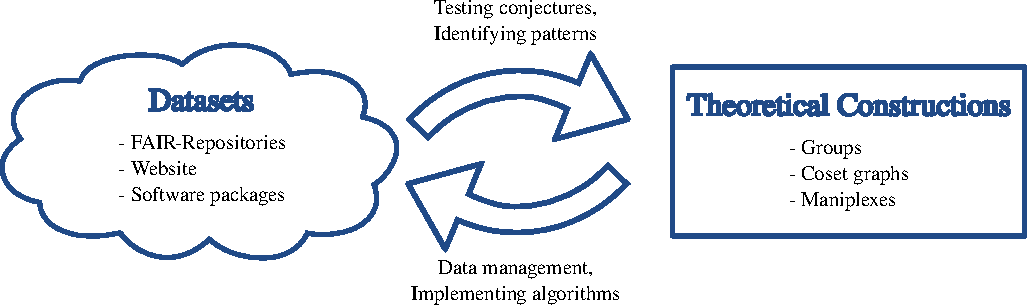
\includegraphics[width=0.9\textwidth]{source/overall}
  \caption{General idea of \ourp\ }\label{fig:idea}
\end{figure}



As a result of the success of our research we will develop a family of repositories, datasets and software packages that allow both researchers and students to experiment, to identify patterns and to formulate conjectures on abstract polytopes.
To achieve this objective, the project will bring together a researcher with expertise on construction of abstract polytopes with prescribed combinatorial conditions with a supervisor with large experience on datasets of discrete objects, in particular of highly symmetric graphs and maps.

\colorrule
\marginLeft{Research objectives}

Abstract polytopes (AP) are combinatorial objects that generalise (the face lattice) of convex polytopes.
Enumeration and classification of highly symmetric convex polytopes goes all the way to the Greeks and the classical problem of classifying what today we know as \emph{Platonic Solids} to the beginning of last century when the classification of higher dimensional convex polytopes was achieved.
By considering combinatorial objects and hence removing the geometric constraints, often imposed by the ambient space, the possibilities for abstract polytopes are now whide open and a complete classification problem turns into a series of enumeration problems of families with particular characteristics.

The degree of symmetry of a polytope can be measured by the number of orbits of its automorphism group on certain substructures called \emph{flags}.
This combinatorial way of measuring symmetry agrees with the classical geometrical notion.
\emph{Regular polytopes} are those that are flag-transitive, meaning they have exactly $1$ flag-orbit.
This \emph{symmetry type} of polytopes has been traditionally the most studied one and includes classical examples as Platonic solids and regular tilings of Euclidean and Hyperbolic spaces.
A slightly less symmetric class of polytopes is that of \emph{$2$-orbit polytopes} and among those, \emph{chiral polytopes} are the most studied.
The notion of chirality is a classical one in other natural sciences, notably in Chemistry.
However, in the context of AP a chiral polytope is one that admits maximal degree of combinatorial rotations but that do not admit mirror reflections.
As I will described in detail below, the classes of regular and chiral polytopes are by far the most studied symmetry types of AP.
This has led to the constructions of some datasets of highly symmetric polytopes, which  shall be described down below.

Chiral polytopes are just one of $2^{n}-1$ possible symmetry types of $2$-orbit $n$-polytopes.
Classical examples of some of the other classes of the $2$-orbit polytopes are known.
However, the general problem of determining if for every pair $(n,T)$ with $n>3$ and $T$ a $2$-orbit symmetry type  exists an $n$-polytope of symmetry type $T$ remains open.
Some examples of maniplexes (a slightly more general class of objects) were build very recently\footcite{PellicerPotocnikToledo_2019_ExistenceResultTwo}, but whether or not they are polytopal remains unknown.
Constructing and classifying $n$-polytopes with $k$-orbits and given symmetry type is still a widely open problem\footcite{CunninghamPellicer_2018_OpenProblems$k$} and it is one of the main motivations for the development of \ourp.

The existing datasets of polytopes suffer of the following restrictions
\begin{enumerate}[label=\textit{(\roman*)}, noitemsep]
  \item They are mainly focused on regular or chiral polytopes.
  \item The size of the examples is very restrictive.
  \item They often exhibit numerous examples of rank $3$ but the amount of examples of rank higher than $4$ drops dramatically.
  \item They are not very user-friendly, either because they exist only as raw data or because the are specific-programming language oriented.
\end{enumerate}

In Table \ref{tab:percentage} we show the proportion of examples according to ranks on the existing datasets of polytopes with examples of rank higher than $3$.


% \begin{center}
\begin{table}
\centering
		\begin{tabularx}{0.7\textwidth}{|\ll{1.5}|\cc{.5}|\cc{.5}|\cc{.5}|}
		\hline
		Dataset & Rank $3$ & Rank $4$ & Rank $\geq 5$ \\ \hline
		Hartley - Regular &
			64.55\%	& 31.61\%	& 3.84\% \\
		Hartley - Chiral &
			85.71\% &	14.29\% &	0.00\% \\
		Conder - Regular&
			61.51\% &	34.70\% &	3.79\% \\
		Conder - Chiral &
			87.01\% &	12.87\% &	0.12\% \\
		Leemans - Regular&
			95.35\% &	4.37\% &	0.30\% \\
		Leemans - Chiral &
			87.82\% &	11.97\% &	0.21\% \\ \hline
		\end{tabularx}
		\caption{Percentages of examples according to rank}\label{tab:percentage}
\end{table}
%   \end{center}

There are two obvious gaps that need to be pushed forward, not necessarily in an independent way, on the process of building new datasets of abstract polytopes: finding examples of higher ranks and building sets that consider different types of symmetries (besides chiral or regular).
With the emerging development of theoretical results for less symmetric polytopes and the need to identify patterns and to find new constructions to attack the numerous open problems related to the existence of polytopes, it is clear that building new datasets of polytopes that overturn the restrictions mentioned above would not only be beneficial but it is almost necessary.

The problematic expressed above outlines our first objective.

\begin{obj}\label{obj:datasets}
  Extend the existing and build new datasets of abstract polytopes and related structures with particular focus on
  \begin{enumerate}[label=\textit{(\roman*)}, noitemsep]
    \item Building examples on ranks higher than $3$
    \item Exploring different symmetry types.
  \end{enumerate}
\end{obj}

\cref{obj:datasets} is of course very general but also very ambitious and should be interpreted as the general research line of \ourp.
Any contribution to this objective is a good way of measuring the overall success of \ourp.

Many of the first datasets of AP are based on the (small) size of the objects.
Either by taking advantage of previously computed objects (such as the library \smallgrp\ ) or by using computational routines that, because of their own nature are limited by the size of the input (such as the \lins).
However, it has been shown that the size of the smallest regular polytope of rank $n$ grows exponentially with $n$\footcite{Conder_2013_SmallestRegularPolytopes}, while the size of the smallest chiral $n$-polytope is at least of factorial growth with respect to $n$\footcite{Cunningham_2017_NonFlatRegular}.
This explains why the amount of examples of higher rank polytopes drops dramatically in the current available datasets.

There is a natural theoretical counterpart to \cref{obj:datasets}, which outlines \cref{obj:theory}:
The lack of datasets AP including other symmetry classes mostly caused by the lack of examples and theoretical constructions of such objects.
Hence, parallel to \cref{obj:datasets} we shall develop the following RO.

\begin{obj}\label{obj:theory}
Develop new constructions of highly symmetric polytopes. In particular, focus on the constructions of abstract regular polytopes with given symmetry type to eventually build the corresponding datasets.
\end{obj}

\cref{obj:theory} by itself represents an extremely ambitious and it goes beyond any two year project.
Any theoretical contribution is already of great interest to the community.
However, we strongly believe that in order to really cause an impact on the workflow of research on abstract polytopes all theoretical contributions should be accompanied by its computational analogue.
As mentioned before, this RO should go parallel to \cref{obj:datasets}, meaning that those theoretical construction should allow us to build new datasets and by exploring those datasets we should be able to identify pattern, formulate conjectures and develop new theoretical constructions.

Another pressing issue to address is that the existent datasets of highly symmetric maps and polytopes are not only limited on size, rank and symmetry type, but they are practically not used.
One of the reasons behind it is that the information in most of these data sets is not very user-friendly.
Even the small amount of existing datasets have been developed by several people, mostly in an independent way, using different notation and different computer algebra systems.
% This usually stops a researcher to use a given data set just because he or she might not be familiar with the notation or programming language.
Moreover, many of these datasets exist only as raw text which is not always easy to consult.
% However, we could use the fact the the amount of data is not huge in our advantage.
This motivates our next RO.

\begin{obj}\label{obj:publish}
% \color{magenta}
% I would change this objective more in the spirit:
Develop standards and a platform for storing and presenting the datasets of abstract polytopes
 (both new and existing) in a unified and user-friendly way, complying with the FAIR principles. In particular:
% \color{black}
% \color{green}
% DELETE: Collect, unify and make the existing data sets user-friendly and in a FAIR-ly way so that \ourp  eventually becomes the standard to-go when consulting or publishing new data on highly symmetric polytopes by
% \color{black}
\begin{enumerate}[label=\textit{(\roman*)}]
%  \item \color{red} **** I would delete this green part. It's too specific: \color{green} Creating and developing a unique data set from the existent ones that unifies notation and identification of the data and make it available so that other researches could experiment and eventually contribute to \ourp .
\item  Survey the existing datasets of AP and related objects, with the emphases on the ways in which they are stored, documented and presented.
\item
Identify the strengths and weaknesses of the existing datasets and propose unified standards for presentation, management and stewardship of the
datasets of AP, following FAIR guideline principles.
% \color{black}
\item Build a web-based and user-friendly interface to datasets of abstract polytopes stored in accordance with the proposed standards.
%  \item \color{red} **** I think that the following two lines could be deleted, as they are in fact subsumed within the development of standards and interface.
%  Developing this data set in a way that can be easily implemented in some of the standards computer algebra systems such as \magma, \gap\ and \sage.
% 	\item Writing appropriate documentation so that \ourp  eventually becomes available for others to contribute.
\end{enumerate}
\end{obj}

\cref{obj:publish} is very concrete and very easy to verify.
It will very easily show progress on \ourp  while at the same time will set a good and concrete step towards our ambitious general objective.

Of course, \ourp  is aimed to become a long term and eventually permanent resource for the community doing research on symmetries of maps and abstract polytopes.
This will not be achievable without the involvement of such community.

\begin{obj}\label{obj:longterm}
Encourage and motivate both well-established and young researchers to use and contribute to \ourp  so that it eventually becomes the standard way to explore, experiment and publish data sets, routines and computational tools for the development of the research of abstract polytopes.
\end{obj}

 \cref{obj:longterm} is very ambitious and we acknowledge that it depends on the community more that on ourselves, but we strongly believe that our approach and the the current status of the could fit together to fill a gap that has been present for many years now.
 We shall achieve this objective by actively consulting an \emph{external committee} of leading experts on the community.


\colorrule

\marginLeft{State of the art}


Enumeration and classification of mathematical objects is a natural way of conducting research.
The discrete nature of combinatorial objects turn them into natural candidates to not only classify families of interesting objects but to enumerate and explicitly list the elements of such families.
This research approach has resulted in the development of interesting data sets of combinatorial objects.
Highly symmetric graphs is arguably the most studied family of combinatorial objects from the approach of building datasets of objects.
It is believed that empirical study of symmetric graphs of small valence started in 1930s, when R.M. Foster began collecting examples of interesting graphs that could serve as models for electrical networks\footcite{Foster_1932_GeometricalCircuitsElectrical}.

% Of course, this area of research has taken advantage of the development and improvement of computational power but the theoretical research goes back to Tutte and his work on classifying $3$-valent arc-transitive graphs\footcite{Tutte_1947_FamilyCubicalGraphs}\footcite{Tutte_1959_SymmetryCubicGraphs} .
% It is believed that empirical study of symmetric graphs of small valence started in 1930s, when R.M. Foster  began collecting examples of interesting graphs that could serve as models.
% His work was published in a book which now carries the name Foster’s census\footcite{Foster_1966_CensusTrivalentSymmetrical}.
The development of the theory, together with more powerful computers, resulted in a breakthrough of datasets of highly symmetric graphs constructions.
Using the classification of automorphism groups of $3$-valent
arc-transitive\footcite{DjokovicMiller_1980_RegularGroupsAutomorphisms} and bitransitive\footcite{Goldschmidt_1980_AutomorphismsTrivalentGraphs} graphs, together with new methods for finding normal subgroups of finite index in a finitely presented group allowed a construction of complete list of all $3$-valent arc-transitive graphs\footcite{ConderDobcsanyi_2002_TrivalentSymmetricGraphs}\footcite{Conder__TrivalentCubicSymmetric}  of order up to $10 000$ vertices, and a list of all $3$-valent bitransitive graph on up to $768$ vertices \footcite{ConderMalnicMarusicPotocnik_2006_CensusSemisymmetricCubic}.
Based on their deep theoretical result on the order of automorphism groups\footcite{PotocnikSpigaVerret_2015_BoundingOrderVertex}, Spiga, Verret and Potočnik compiled a complete list\footcite{PotocnikSpigaVerret_2015_Census4Valent}  of all trivalent vertex-transitive graphs of order at most $1280$.
Very recently, using the database of vertex-transitive groups of small degree, Conder and Verret have compiled a complete list of all edge-transitive graphs (of arbitrary valence) up to order $63$ \footcite{ConderVerret_2019_EdgeTransitiveGraphs}, while
Holt and Royle have extended their census of all vertex-transitive graphs up to order $48$\footcite{HoltRoyle_2020_CensusSmallTransitive}.

% The classification and enumeration of groups has been also an intriguing problem since the beginning of theory.
% In 1854 Cayley\footcite{Cayley_1854_Vii.TheoryGroups} introduced the axiomatic definition of a group and enumerated the groups of order up to $6$.
% Of course this is just the first step in what became an active research in both, theoretical mathematics\footcite{BlackburnNeumannVenkataraman_2007_EnumerationFiniteGroups} , as well as a motivation to develop computation tools such as the library \smallgrp \footcite{BescheEickOBrien_2001_GroupsOrderMost} of small groups of \gap\ .
% In fact, one of the principal motivators on the study of symmetries of discrete objects the the \emph{classification of Finite Simple Groups}. It turns out that many of the so-called sporadic simple groups can be understood as symmetry groups of discrete objects.
% This classification eventually derived in the construction of the \textsc{Atlas} of Finite Groups \footcite{Conway_1986_AtlasFiniteGroups}.

% \colorrule


% ****OLD STUFF*********
% \marginLeft{Once upon a time of polytopes}
% The term “polytope” is the generic word to refer to classical geometrical objects such as polygons and polyhedra; while maps on surfaces are also geometrical and topological objects that share many properties with classical convex polyhedra. Abstract polytopes are purely combinatorial objects that generalise the geometrical notion of convex polytopes while maniplexes are a further generalisation of abstract polytopes. The most relevant shared property for the objects of our interest is symmetry, which sits our project in the interplay between combinatorics and group theory with a natural flavor of geometry and topology. We introduce below the mathematical context of the objects that we are interested in. We decide to use an historical approach to emphasise on the relevance of such objects across the development mathematical knowledge.
% *********************************************

The problem of enumerating and classifying regular polyhedra in the Euclidean space is as old as formal mathematics themselves.
The enumeration and classification of the five Platonic Solids is one the most antique classification problems.
For many years it was considered a complete classification problem (and it was) but later it was shown that by relaxing geometrical constraints we could generalise platonic solids to stellated polyhedra\footcite{Kepler_1864_HarmoniaMundiOpera}\footcite{Poinsot_1810_MemoireSurLes}\footcite{Cauchy_1813_AlCauchyRecherche}, \emph{infinite skew polyhedra}\footcite{Coxeter_1937_RegularSkewPolyhedra} and finally to \emph{Grünbaum-Dress polyhedra}\footcite{Gruenbaum_1977_RegularPolyhedraOld}\footcite{Dress_1981_CombinatorialTheoryGrunbaums}\footcite{Dress_1985_CombinatorialTheoryGrunbaums}, which is what today is accepted as the complete classification of regular polyhedra in the Euclidean space\footcite{McMullenSchulte_1997_RegularPolytopesOrdinary}.
% There is archaeological evidence of stone balls representing what we now know as  the symmetry groups of the five Platonic Solids.
% This evidence was discovered in Scotland and dates from the first half of the third millennia BCE.
% It is also known that the Egyptians and Babillonials were aware of the existence of such object but undoubtedly the Greeks have the credit of studying them form a purely mathematical interest.
% In fact, the thirteenth book of Euclid’s Elements is devoted to the classification of the five Platonic Solids.
% % A classification problem often relates to the definition of the objects that are being classified.
% By relaxing geometrical conditions on the definition of polyhedra, new objects emerged.
% In a paint from 1420 by Paolo Uccello and an engraving from 1568 by Wenzel Jamnitzer appear the oldest representation of what we know as \emph{regular stellated polyhedra}.
% % These are objects that share many properties with platonic solids but have the special characteristic of having stellated polygons as face s.
% These polyhedra were rediscovered by Kepler in the late 1500’s and then by Poinsot in 1809.
% % who also discovered their duals; both authors described them with a mathematical approach.
% Soon later, in 1811 Cauchy show that the four objects described by Poinsot were the only possible \emph{regular stellated polyhedra}.
% The theory of polyhedral-like structures took a complete new breath with the contributions of H.S.M. Coxeter.
% Coxeter's monograph\footcite{Coxeter_1973_RegularPolytopes} on regular polytopes is most likely its most influential publication, but some of his remarkable contributions date as early as 1937 when together with J.F. Petrie described the \emph{regular skew polyhedra}\footcite{Coxeter_1937_RegularSkewPolyhedra} as infinite analogues of Platonic solids.
% By relaxing the definition of a regular polyhedron Grünbaum presented\footcite{Gruenbaum_1977_RegularPolyhedraOld} a list of $47$ regular polyhedra which included the Platonic Solids, Stellated polyhedra as well as Petrie-Coxeter skew polyhedra.
% Soon after A. Dress describes\footcite{Dress_1981_CombinatorialTheoryGrunbaums} another polyhedron and proves\footcite{Dress_1985_CombinatorialTheoryGrunbaums} that the list of $48$ regular polyhedra in the Euclidean space is complete.

 B.Grünbaum was one of the firsts that formally treated geometrical polyhedra-like objects as purely combinatorial objects by introducing the notion of the notion \emph{polystroma}\footcite{Gruenbaum_1978_RegularityGraphsComplexes}.
This notion eventually evolved to what we know today as \emph{abstract polytopes}, introduced in the early 80's
\footcite{Schulte_1980_RegulareInzidenzkomplexe_PhDThesis}%\footcite{DanzerSchulte_1982_RegulareInzidenzkomplexe.I}\footcite{Schulte_1983_RegulareInzidenzkomplexe.Ii} .

The theory of highly symmetric abstract polytopes nourishes from several branches of mathematics, including group theory, topology and geometry.
Coxeter is also attributed to classify the groups generated by hyperplane reflections, leading to what we today know as \emph{Coxeter groups}.
% Coxeter groups have an influential role in several branches of mathematics.
They of course, appear as the symmetry groups of regular polytopes and tessellations of the Euclidean and Hyperbolic spaces\footcite{Humphreys_1990_ReflectionGroupsCoxeter}, but they have made their way to Tits geometries\footcite{Tits_1974_BuildingsSphericalType}, computational Lie group theory, Hecke algebras\footcite{Cohen_1991_CoxeterGroupsThree}, just to mention some.

In 1978 G. Jones and D. Singerman published his classical manuscript\footcite{JonesSingerman_1978_TheoryMapsOrientable} which settle the necessary theory to identify maps on orientable surfaces with what in modern terminology we called its \emph{monodromy group}.
The ideas behind this paper show important equivalences between topological maps (embedding of graphs on orientable surfaces), certain quotients triangular groups (Coxeter groups of rank $3$), maps on Riemann surfaces and certain permutations on the darts of the map.
These equivalences are a combinatorial/discrete version of the classical Uniformization theorem\footcite{Abikoff_1981_UniformizationTheorem} for Riemann surfaces.
The work of Jones and Singerman was an important contribution on the theory of discrete group actions on Riemann surfaces and it was eventually connected the theory Grothendieck's \emph{Dessins d'enfant}\footcite{JonesWolfart_2016_DessinsDenfantsRiemann}.
% Some other combinatorial equivalences of maps on surfaces were also explored by Tutte\footcite{Tutte_1973_WhatIsMap}, Vince\footcite{Vince_1983_CombinatorialMaps}  and  Wilson\footcite{Wilson_2012_ManiplexesPart1}.

% % Coxeter's work serve as inspiration for many mathematicians, one of them being , which is an ancestor of what we today call \emph{abstract polytopes}.
% % Grünbaum is also responsible of first treating symmetric polyhedra from a combinatorial viewpoint.
% By relaxing the definition of a regular polyhedron he presented\footcite{Gruenbaum_1977_RegularPolyhedraOld} a list of $47$ regular polyhedra which included the Platonic Solids, Stellated polyhedra as well as Petrie-Coxeter skew polyhedra. Soon after A. Dress describes\footcite{Dress_1981_CombinatorialTheoryGrunbaums} another polyhedron and proves\footcite{Dress_1985_CombinatorialTheoryGrunbaums} that the list of $48$ regular polyhedra is complete.
% The central class of objects in \ourp is that of \emph{highly symmetric abstract polytopes}.
% Abstract polytopes were introduced by Schulte in his PhD thesis\footcite{Schulte_1980_RegulareInzidenzkomplexe_PhDThesis} and he also established most of the early results.
% Abstract polytopes are a particular class of partially ordered sets that combinatorially generalise the (face-lattices) of convex polytopes but also include the incidence structure of many other geometrical objects such as tilings of $\bE^{n}$ and $\bH^{n}$ as well as most maps on surfaces.
% Early research focused on \emph{regular polytopes}, that is, those with the highest degree of symmetries.
%  being one the most remakable results the correspondence between regular polytopes and \emph{string C-groups}, that is smooth quotients of Coxeter groups that satisfy the Intersection Property\footcite{DanzerSchulte_1982_RegulareInzidenzkomplexe.I}\footcite{Schulte_1983_RegulareInzidenzkomplexe.Ii}\ .

% The correspondence between regular polytopes and its automorphism group made possible turn the combinatorial problem of building regular polytopes into a group theoretical problem. This approach has been the standard techinque to build regular polytopes and it would be impossible to list them all.
Abstract polytopes include many of the object mentioned above.
Regular abstract polytopes, those with larger degree of symmetry are by far the most studied class of abstract polytopes.
Most of this early theory can be found in the very dense and comprehensive monograph written by Schulte a McMullen\footcite{McMullenSchulte_2002_AbstractRegularPolytopes}.
Of our particular interest is the problem of building regular polytopes, for which numerous publications exists.
We should mention that there exist universal constructions%
\footcite{Schulte_1983_ArrangingRegularIncidence}\footcite{Schulte_1985_ExtensionsRegularComplexes}, %
constructions prescribing local combinatorics \footcite{Danzer_1984_RegularIncidenceComplexes}\footcite{ Pellicer_2009_ExtensionsRegularPolytopes} %\footcite{ Pellicer_2010_ExtensionsDuallyBipartite}
and constructions fixing interesting families of groups as automorphism groups\footcite{CameronFernandesLeemansMixer_2017_HighestRankPolytope}\footcite{FernandesLeemans_2018_CGroupsHigh}\footcite{ LeemansMoerenhoutOReillyRegueiro_2017_ProjectiveLinearGroups}\footcite{ Pellicer_2008_CprGraphsRegular} .

The second most studied symmetry class of polytopes is that of \emph{chiral polytopes}.
% Informally speaking, a chiral polytope is a polytope having full degree of (combinatorial) rotational symmetry without having (combinatorial) reflections.
They were introduced by Schulte and Weiss in 1990\footcite{SchulteWeiss_1991_ChiralPolytopes}
%  where an analogous result to the one for the automorphism group of regular polytopes was established.
% Chiral polytopes were introduced
as a natural generalization of \emph{chiral maps}, which have been part of the classical theory of maps from it begging and numerous examples exist\footcite{CoxeterMoser_1972_GeneratorsRelationsDiscrete}\footcite{ConderDobcsanyi_2001_DeterminationAllRegular}\footcite{Sherk_1962_FamilyRegularMaps} .
However, the problem of constructing chiral polytopes of higher ranks has proved to be much harder to that of constructing regular polytopes.
Some rank $4$ examples were constructed as quotients of hyperbolic tilings\footcite{NostrandSchulteWeiss_1993_ConstructionsChiralPolytopes}\footcite{SchulteWeiss_1994_ChiralityProjectiveLinear}\footcite{Nostrand_1994_RingExtensionsChiral}\footcite{NostrandSchulte_1995_ChiralPolytopesHyperbolic} .
A universal construction\footcite{SchulteWeiss_1995_FreeExtensionsChiral} was used to produce the first (infinite) example of a rank-$5$ chiral polytope.
However, the first finite rank $5$ polytopes were constructed by Conder et al. in 2008\footcite{ConderHubardPisanski_2008_ConstructionsChiralPolytopes}.
It was until 2010 that Pellicer showed\footcite{Pellicer_2010_ConstructionHigherRank} the existence of chiral polytopes of rank $n$ for ever $n \geq 4$;
The result by Pellicer, although constructive, is not very practical. The size of his examples grow as a tower of exponential functions with length depending on $n$.
Later on examples of new chiral polytopes have been constructed from previously known ones\footcite{CunninghamPellicer_2014_ChiralExtensionsChiral}\footcite{ConderZhang_2017_AbelianCoversChiral}\footcite{Montero_2019_ChiralExtensionsToroids_PhDThesis}\footcite{Montero_2021_SchlaefliSymbolChiral} .

The problem of classifying and enumerating highly symmetric polytopes has been part of the theory from the beginning.
% Even before the emergence of computers appeared the first
% From classification of the $5$ Platonic Solids to the enumeration of the $48$ Grünbaum-Dress polyhedra in $\bE^{3}$ depend on strong geometric restrictions.
% However, the combinatorial nature of abstract poltypes open the possibilities to, in principle, have numerous examples of abstract polytopes.
These has lead to the construction of some datasets of highly symmetric polytopes, which we review below.

\paragraph{Conder - Regular orientable maps by genus} Computed by M. Conder it originally contained all ($3378$) regular maps on orientable surfaces of genus 2 to 101 up to isomorphism an duality. It was later extended to include genus up to $301$ for a total of $15824$ maps.
Computed with the help of \lins routine of \magma and published as raw text.

\paragraph{Conder - Regular non-orientable maps by genus} Every map on a non-orientable surface admits an orientable double cover. Conder used this fact to originally compute all ($862$) non-orientable regular maps of genus $2$ to $202$ and then extended to genus up to $602$ for a total of $3260$ maps.
Computed with the help of \lins routine of \magma and published as raw text.

\paragraph{Conder - Chiral maps by genus } Census containing all ($594$) chiral maps on orientable surfaces of genus $2$ to $101$. This census was later extended to genus up to $301$ for a total of $3870$.
Computed with the help of \lins routine of \magma and published as raw text.
%
\paragraph{Conder - Rotary maps by size} This census contains all rotary (that is regular or chiral) maps whose rotation group has less than $2000$ elements (equivalently, such that the map has less than $1000$ edges).
Computed with the help of \lins routine of \magma and published as raw text. There exist versions of this census containing only regular and only chiral maps.
%
\paragraph{Potocnik - Regular maps by size} An improvement on Conder's census containing all ($255,980$) regular maps whose automorphism group is of order less than $6,000$ for orientable maps and $3,000$ for non-orientable maps. Published as \magma files available to download with a CVS-file of precomputed information.
%
\paragraph{Potocnik - Chiral maps by size} An analogous to the one above but for chiral maps. It contains a total of $122,092$ chiral maps whose automorphism group has order less than $6,000$.

\paragraph{Hartley - The Atlas of Small Regular Polytopes } It was build using \smallgrp routine of \gap\ and contains all regular polytopes with at most $2000$ flags, except those of size $1024$ and $1536$. It contains $9212$ examples. They are presented in a nice web interface and the code is available to download.

\paragraph{Hartley - The Atlas of Small Chiral Polytopes} Every chiral polytope admits a minimal regular cover. Hartley used this fact to compute the first atlas of chiral polytopes. This dataset consists of all chiral polytopes whose minimal regular cover belongs to the Atlas of Small Regular Polytopes. This gave a total of $48$ chiral polytopes of rank $3$ and $8$ polytopes of rank $4$.

\paragraph{Conder - Regular polytopes up to 2,000 flags} A dataset containing, up to duality, all ($5809$) regular polytopes with at most $2000$ flags (which is the same as the order of the automorphism group).

\paragraph{Conder - Chiral polytopes up to 2,000 flags} A dataset containing, up to duality, all ($839$) chiral polytopes with at most $2000$ flags (which is the twice the order  of the automorphism group).


\paragraph{Leemans et al. - An Atlas of polytopes for small simple groups} This is an ongoing atlas that contains regular polytopes whose automorphism group is an almost simple group. It currently contains $55,575$ regular polytopes. The atlas is presented on a website with downloadable data.

\paragraph{Leemans et al. - An Atlas of chiral polytopes for small simple groups} It is the analogous to the one above but for chiral polytopes. It currently contains a total of $19,964$ polytopes.

% As mentioned before, the existing datasets of polytopes






% \parskip
% \subsubsection*{Problem identification and Research and Innovation objectives.}
%
% These existing datasets of polytopes suffer of the following restrictions
% \begin{enumerate}[label=\textit{(\roman*)}, noitemsep]
%   \item They are mainly focused on regular or chiral polytopes.
%   \item The size of the examples is very restrictive.
%   \item They often exhibit numerous examples of rank $3$ but the amount of examples of rank higher than $4$ drops dramatically.
%   \item They are not very user-friendly, either because they exist only as raw data or because the are specific-programming language oriented.
% \end{enumerate}
%
% As explained before, most of the existent datasets of polytopes are either completely focused on $3$-polytopes (maps) or have very little examples of higher ranks.
% In Table \ref{tab:percentage} we show the proportion of examples according to ranks.
%
%
% % \begin{center}
% \begin{table}
% \centering
% 		\begin{tabularx}{0.7\textwidth}{|\ll{1.5}|\cc{.5}|\cc{.5}|\cc{.5}|}
% 		\hline
% 		Dataset & Rank $3$ & Rank $4$ & Rank $\geq 5$ \\ \hline
% 		Hartley - Regular &
% 			64.55\%	& 31.61\%	& 3.84\% \\
% 		Hartley - Chiral &
% 			85.71\% &	14.29\% &	0.00\% \\
% 		Conder - Regular&
% 			61.51\% &	34.70\% &	3.79\% \\
% 		Conder - Chiral &
% 			87.01\% &	12.87\% &	0.12\% \\
% 		Leemans - Regular&
% 			95.35\% &	4.37\% &	0.30\% \\
% 		Leemans - Chiral &
% 			87.82\% &	11.97\% &	0.21\% \\ \hline
% 		\end{tabularx}
% 		\caption{Percentages of examples according to rank}\label{tab:percentage}
% \end{table}
% %   \end{center}
%
% There are two obvious gaps that need to be pushed forward, not necessarily in an independent way, on the process of building new datasets of abstract polytopes: finding examples of higher ranks and building sets that consider different types of symmetries (besides chiral or regular).
% With the emerging development of theoretical results for less symmetric polytopes and the need to identify patterns and to find new constructions to attack the numerous open problems related to the existence of polytopes, it is clear that building new datasets of polytopes that overturn the restrictions mentioned above would not only be beneficial but it is almost necessary.
%
% The problematic expressed above outlines our first objective.
%
% \begin{obj}\label{obj:datasets}
%   Extend the existing and build new datasets of abstract polytopes and related structures with particular focus on
%   \begin{enumerate}[label=\textit{(\roman*)}, noitemsep]
%     \item Building examples on ranks higher than $3$
%     \item Exploring different symmetry types.
%   \end{enumerate}
% \end{obj}
%
% \cref{obj:datasets} is of course very general but also very ambitious and should be interpreted as the general research line of \ourp.
% Any contribution to this objective is a good way of measuring the global success of \ourp.
%
% % The general objective of \ourp  is to build a environment of data sets and computational tools for maps, abstract polytopes and maniplexes.
% % We expect this environment to be not only of the interest but more importantly, useful to the community doing research on this area.
% % In the following paragraphs, we explain how we split this general objective into several particular and very concrete objectives.
% Another pressing issue to address is that the existent datasets of highly symmetric maps and polytopes are not only limited in the sense discussed above, they have not been exploded to its full capacity.
% One of the reasons behind it is that the information in most of these data sets is not very user-friendly.
% Even the small amount of existing data sets have been developed by several people, mostly in an independent way, using different notation and different computer algebra systems.
% % This usually stops a researcher to use a given data set just because he or she might not be familiar with the notation or programming language.
% Moreover, many of these datasets exist only as raw text which is not always easy to consult.
% % However, we could use the fact the the amount of data is not huge in our advantage.
%
%
% \begin{obj}\label{obj:publish}
% Collect, unify and make the existing data sets user-friendly and in a FAIR-ly way so that \ourp  eventually becomes the standard to-go when consulting or publishing new data on highly symmetric polytopes by
% \begin{enumerate}[label=\textit{(\roman*)}, noitemsep]
%  \item Creating and developing a unique data set from the existent ones that unifies notation and identification of the data and make it available so that other researches could experiment and eventually contribute to \ourp .
% \item Building a web-based interface to our data set for easy and quick consultation.
%  \item Developing this data set in a way that can be easily implemented in some of the standards computer algebra systems such as \magma, \gap and \sage.
% 	\item Writing appropriate documentation so that \ourp  eventually becomes available for others to contribute.
% \end{enumerate}
% \end{obj}
%
% \cref{obj:publish} is very concrete and very easy to verify. It very easily show progress on \ourp  while at the same time sets a good start point to our ambitious general objective.
% The current state-of-the-art allows us to start with  from the very beginning of \ourp
%
% Many of the first data sets of abstract polytopes are based on the (small) size of the objects.
% Either by taking advantage of previously computed objects (such as the library \smallgrp) or by using computational routines that, because of their own nature are limited by the size of the input (such as the \lins).
% However, it has been shown that the size of the smallest regular polytope of rank $n$ grows exponentially with $n$\footcite{Conder_2013_SmallestRegularPolytopes} , while the size of the smallest chiral $n$-polytope is at least of factorial growth with respect to $n$\footcite{Cunningham_2017_NonFlatRegular}.
% This explains why the amount of examples of higher rank polytopes drops dramatically on the current available datasets.

% On the other hand, there are interesting infinite families (eg. toroids\footcite{CollinsMontero_2021_EquivelarToroidsFew} ) or constructions (eg. pyramids, prisms\footcite{GleasonHubard_2018_ProductsAbstractPolytopes}, antiprisms\footcite{GleasonHubard_2021_AntiprismAbstractPolytope}, generalised cubes and extensions\footcite{Danzer_1984_RegularIncidenceComplexes}\footcite{Pellicer_2009_ExtensionsRegularPolytopes} \footcite{Cunningham_2021_FlatExtensionsAbstract}\footcite{Montero_2021_SchlaefliSymbolChiral} ) that can be easily implemented to build datasets of higher ranks and interesting symmetry types.
% Motivated from the previous discussion we propose our next objective.
%
% \begin{obj}\label{obj:constructions}
% Explore the literature and implement appropriate routines to construct new examples of polytopes from previously known ones.
% \end{obj}
%
% \cref{obj:constructions} is very practical and it comes alongside withits theoretical parallel wich, just by its relevance\footcite{CunninghamPellicer_2018_OpenProblems$k$} presents the most ambitious objective of this proposal.

% The lack of not only datasets but also theoretical constructions of certain symmetry types for polytopes motivates the following objective.
%
% \begin{obj}\label{obj:theory}
% Develop new constructions of highly symmetric polytopes. In particular, focus on the constructions of abstract regular polytopes with given symmetry type to eventually build the corresponding data sets.
% \end{obj}
%
% \cref{obj:theory} by itself represents an extremely ambitious and it goes beyond any two year project.
% Any theoretical contribution is already of great interest to the community.
% However, we strongly believe that in order to really cause an impact on the workflow of research on abstract polytopes all theoretical contributions should be accompanied by its computational analogue.
%
% Of course, \ourp  is aimed to become a long term and eventually permanent resource for the community doing research on symmetries of maps and abstract polytopes.
% This will not be achievable without the involvement of such community.
%
% \begin{obj}\label{obj:longterm}
% Encourage and motivate both well-established and young researchers to use and contribute to \ourp  so that it eventually becomes the standard way to explore, experiment and publish data sets, routines and computational tools for the development of the research of abstract polytopes.
% \end{obj}
%
%  \cref{obj:longterm} is very ambitious and we acknowledge that it depends on the community more that on ourselves, but we strongly believe that our approach and the the current status of the could fit together to fill a gap that has been present for many years now.
% It is important to remark that the community has faced a similar scenario before.
% Many of the early research on abstract polytopes was collected on the comprehensive manuscript\footcite{McMullenSchulte_2002_AbstractRegularPolytopes}  and nowadays it serves as a natural and standard theoretical reference.
% Our expectations is that \ourp  eventually becomes the computational analogue for our community.
% %%% OVERVIEW %%%
% \marginLeft{Overview}%


%%% 1.1.2 STATE-OF-THE-ART %%%
% \colorrule
% \marginLeft{State-of-the-art}%
%
%
%
% %%% 1.1.3 OBJECTIVES %%%
% \colorrule
% \marginLeft{Objectives}%
% \textbf{Lorem ipsum dolor sit amet}, consectetur adipiscing elit, sed do eiusmod tempor incididunt ut labore et dolore magna aliqua. Ut enim ad minim veniam, quis nostrud exercitation ullamco laboris nisi ut aliquip ex ea commodo consequat.
% \begin{itemize}[leftmargin=*, noitemsep,topsep=0pt]
%     \item \textbf{Duis aute irure dolor in reprehenderit in voluptate velit.} \marginRight{obj 1}
%     \item \textbf{Ut enim ad minim veniam}, quis nostrud exercitation ullamco. \marginRight{obj 2}
% \end{itemize}
% Quis autem vel eum iure reprehenderit qui in ea voluptate velit esse quam nihil molestiae consequatur, vel illum qui dolorem eum fugiat quo voluptas nulla pariatur?
%
% %%% 1.1.4 ORIGINALITY %%%
% \colorrule
% \marginLeft{Originality}%
% Sed ut perspiciatis unde omnis iste natus error sit voluptatem accusantium doloremque laudantium, totam rem aperiam, eaque ipsa quae ab illo inventore veritatis et quasi architecto beatae vitae dicta sunt explicabo. Nemo enim ipsam voluptatem quia voluptas sit aspernatur aut odit aut fugit, sed quia consequuntur magni dolores eos qui ratione voluptatem sequi nesciunt.

% \paragraph{Historical remarks}.
% Highly symmetric polyhedra have captivated humankind for almost as long as history itself.
% The period succeeding the Greeks goes to the Roman and eventually the Byzantine empire, whose attitude to mathematics (and to other sciences as well) was ambiguous going form encouragement to suppression. However they must be credited by preserving the Greek’s mathematical knowledge. The Arabs did many contributions to mathematics in this period, however it seems that geometry and hence symmetric objects was not of their scientific interest. However, they did have a strong empirical knowledge of symmetry. It is possible to find patterns in the Alhambra that exemplify many of what we know today as the planar crystallographic groups, which are closely related to the symmetry groups of highly symmetric polyhedra.
% This takes us to the middle ages where as in other sciences, mathematical knowledge was not of heavy interest. However again the notion of symmetry did developed through artistic pieces. Notably, the oldest appearances of what we today know as stellated polyhedra appeared in a paint from 1420 by Paolo Uccello and an engraving from 1568 by Wenzel Jamnitzer. These objects were rediscovered first by Kepler in the late 1500’s and then by Poinsot in 1809; both of which described them with a mathematical approach. Soon later, in 1811 these objects where classified by Cauchy.
% Although Platonic solids are as old as mathematics themselves, their theoretical relevance did not develop the same way as some other aspects of mathematics. It was not until the second half of the 19th century that Schäfli formally studied the symmetries of Platonic Solids and their higher dimensional analogous, those that we today know as regular convex polytopes. To this point it is important to remark that geometrical properties of convex polytopes allow us to fully classify them combinatorially by a sequence of numbers, the Schläfli symbol (explained in detail below), and hence their reconstruction from a computational viewpoint is extremely simple.
% The theory of polyhedral-like structures took a complete new breath with the contributions of H.S.M Coxeter. Those contributions are extremely numerous to list in here and spread al along the 20th century. However, we should mention that Coxeter formally brought together the interplay between symmetry (group theory and geometry) and combinatorial objects. One of his most remarkable contributions is that of classifying symmetry groups generated by reflections (known today as Coxeter groups).  The impact of Coxeter’s contributions has served not only as reference but also as inspiration of many distinguished mathematicians and impacted not only to the community working with highly symmetric discrete objects but also to a huge extend of subareas of modern mathematics, just to mention some of them we refer to the work by Grünbaum and Dress who settle the first steps to what we today call abstract polytopes, and to the work by Tits on buildings  and its further generalisation by Buekenhout as diagram geometries, both of which are related to the understanding of some of the so called sporadic almost simple groups.
%
% \paragraph{Maps on surfaces.}
% % \marginLeft{Maps on surfaces}.
% A map M on a surface S can be though as an embedding of a graph G on a surface such that the faces (connected components S ) are homeomorphic to discs. The group Aut(M) of automorphisms of the map can be understood as the group of automorphism of G that extend to homeomorphisms of S. This allows us to understand the surface in a combinatorial way. Moreover, the baricentric subdivision of the map induces a triangulation of the surface into flags (figure?) so that the the action of Aut(M) on the set of flags is free. This implies that we can understand Aut(M) as a fixed-point free permutation group on the set of flags. Whenever this action is transitive the map is called regular (reflexible). This is consistent with the notion of regularity of polyhedra introduced by [REF]. In a regular map M, all the faces have the same amount p of vertices at its boundary and each vertex have the same degree q. In this situation we say that M is of (Schläfli) type {p,q}. Informally speaking, a regular map is one that admits fully reflectional symmetry. A regular map of type {p,q} is fully determined by its automorphism group and moreover, this automorphism group is a quotient of the Coxeter group [p,q]. This fact has been heavily exploited to build data sets of regular maps. Currently, there are several data sets of regular maps available. The approach taken on the development of each of them differ slightly one from another. We list the available data below.
% In [C2006ROM101] Conder lists all the regular maps on orientable surfaces of genus 2 to 101 (3378 entries); this census was later improved in [C2011 ROMg301] to list all regular orientable maps of genus 2 to 301. The census [C2011ROMg301] has 15824 entries. Every non-orientable regular maps admit an regular orientable double cover, as a consequences the previous cenci automatically have their non-orientable analogous: [C2006RNOMg202] and [C2011RNOMg602] which list the regular non-orientable maps of genus 2 to 202 (862 entries) and of genus 2 to 602 (3260). The data sets described above were computed using the LowIndexNormalSubgroups of MAGMA. Further uses of this routine lead to the data sets [C2012RMe1000] of regular (orientable and non-orientable) maps with at most 1000 edges.
% A regular map on an orientable surface  admits an index-two subgroup of automorphisms inducing full rotational symmetry. The maps (regular or not) admitting this high degree of rotational symmetry are often call rotary maps and such maps can divided in two classes: reflexible (what we before called regular) and irreflexible or chiral. Rotary maps are often regarded as the most symmetric maps, since many authors are only interested in orientation-preserving automorphisms. The rotation group of a rotary map of type {p,q} is a quotient of$ [p,q]{+}$, the even subgroup of the Coxeter Group [p,q] by a normal subgroup M of [p,q]+. If M is normal not only in $[p,q]{+}$ but also in [p,q], then the associated rotary map is regular, otherwise is chiral.  This fact has been used to build families of rotary maps and some data sets of such have been built as well. Notably, in [C2012RotM1000e] Conder lists all the rotary maps with up to 1000 edges while in  [P2014RotM3000e] Potočnik impoves this dataset by listing all rotary maps with up to 3000 edges (255,980 entries). Both datasets include a version where only regular or only chiral maps are listed. In [C2006ChiM101g] Conder presents a census of  chiral  maps on orientable surfaces of genus from 2 to 101 (594 entries). This  census was later improved by Conder and in [C20014ChiM301g] he presents the list of the 3870 chiral maps on orientable surfaces of genus from 2 to 301.
%
% \paragraph{Abstract polytopes.} An abstract polytope is a partially ordered set that shares many properties with the face-lattice of a convex polytopes. Examples of such are, of course (the face lattices of), all convex polytopes but also tilings of Euclidean and hyperbolic spaces, maps on surfaces as well as many objects with in principle, not necessarily nice geometrical representation. In a bit more detailed way, an abstract polytope (n-polytope, for short) is a combinatorial generalisation of all such geometrical objects. Most maps on surfaces are 3-polytopes and every 3-polytope can be regarded as a map on a not necessarily compact surface. The notion of flags extend in a natural from maps to n-polytopes as maximal chains of the poset containing exactly one face of each of the  n possible ranks (dimensions). Each flag F has a unique i-adjacent flag Fi that shares all the faces but the one of rank i. This notion of adjacency of flags turns the set of flags into a n-edge coloured graph, the flag graph of the polytope. The group of automorphism of a polytope is the group of colour-preserving automorphisms of the flag graph. This is in fact isomorphic to the automorphism group of P as poset, namely, the set of order-preserving bijections and also coincide with the topological definition of automorphisms for maps. The degree of symmetry of a polytope can be measured with the number of falg-orbits of the automorphism group. As with maps, a polytope is regular if it is transitive on flags; regular polytopes are the most symmetric ones. The automorphism group of a regular polytope is a quotient of a Coxeter group with string diagram. As before, this result has been extensively used to build regular polytopes from a theoretical approach. However, the amount of datasets available regular n-polytopes, with n >= 4 is significantly small compared to that for maps. In [H2006RP2000f] Hartley lists all the possible regular polytopes with at most 2000 flags, excetp those with 1024 or 1536 flags). He used the library of small groups of GAP, that lists contains all possible groups with at most 2000 elements. The census [C2012RP2000f] containing essentially the same information was computed by Conder. There are some datasets containing all regular polyopes whose automorphism group belongs to a relevant family of groups. Notably Hartley’s [HRPSSG] contains the regular polytopes whose automorphism group is one of the sporadic symple groups of order smaller thant that of the Held group (aprox. 4X109). While in [LRPASG] Leemans keeps an on going census of regular polytopes whose automorphism group is an almost simple group. Both data sets offer several thousands of examples of regular polytopes but most of them (over 90%) are rank 3 polytopes (maps).
% In a very similar ways as with maps, there is a combinatorial definition of rotary n-polytopes. Rotary but non-regular polytopes are called chiral and besides regular polytopes. Chiral polytopes have 2-flag orbits and the class of chiral polytopes is the second most studied symmetry family of abstract polytopes. However, the availability of data sets or even explicit examples of chiral polytopes of rank higher than 4 is almost non-existent. Chiral polytopes of rank 3 (chiral maps) are a classical part of the theory and the definition naturally extends to higher ranks. Chiral polytopes were formally introduced by Schulte and Weiss in beginning of the 90’s [REF!] and for many years it was hard to theoretically find examples of chiral polytopes of rank 4 or 5. Moreover, in the attempt of finding such examples many non-existence results were established. It was until 2010 that Pellicer proved that chiral n-polytopes exists for any n [REF]. Pellicer’s proof is constructive but trying to compute the smallest of his examples of rank larger than 10 is not practical with the current computational power; the size of such polytopes grows as a tower of exponential functions whose length grows with n.
% As mentioned before the existence of data sets of chiral polytopes is very limited. Every chiral polytope admits a minimal regular cover, which implies that we can explore the data sets of regular polytopes and check which of them are regular covers of chiral polytopes. Using this approach, Hartley collected in [HSCP] all the chiral polytopes whose minimal regular cover appears in [H2012RP2000f]. This census of chiral polytopes contains only 56 polytopes (compared to the over 20 000 entries in the census of regular polytopes used to build it). Moreover, only 8 of such polytopes are of rank 4, the remaining 48 are chiral maps. Using LowIndexNormalSubgroups routine for MAGMA , Conder constructed the census [CCP2000f] which contains all chiral polytopes with at most 2000 flags. To no one surprise, this atlas contains mostly examples in rank 3, a few examples in rank 4 and just one example in rank 5. As with regular polytopes. Leemans et al. Keep in [LCPASG] a on going census of chiral polytopes whose automorphism group is one of the almost simple groups. This census contains just a few thousands of entries and as with the other cenci of chiral polytopes, the vast majority of them are or rank 3, whit not a single example of rank larger than 5.
% Chiral polytopes are just one of (2n) -1 possible symmetry type class of 2-orbit polytopes. Classical examples of some of the other classes of 2-orbit polytopes are known. However, the general problem of determining if for every pair (n,T) with n >3 and T a symmetry type of 2-orbit polytopes exists an n-polytope of symmetry type T remains mostly open. Of course, collecting and classifying known examples and constructions is of the interest of the community and it might help to solve existence problems as the one just presented.
% Constructing and classifying n-polytopes with k-orbits and given symmetry type is an fairly recent and active research area and just as with more symmetric polytopes, trying to identify patterns and  constructing new examples from previously known examples could be seriously improved by the construction of data sets of polytopes.  Some of the possible uses will be discussed below.
%
% Maniplexes. We very briefly mention the notion of an n-maniplex. Roughly speaking, a maniplex is a combinatorial generalization of both maps and (the flag graph of) polytopes. They were introduced by Wilson in [REF] but have been gaining popularity recently. In particular, the usage of maniplexes has allowed to use graph-theoretical techniques to build polytopes [REF! PrimozMicaelDanie, Tero, Elias, EliasIsaTero, Gabe]. Highly symmetric maniplexes that are not polytopes seem to be very degenerate. Moreover, there is a characterisation of maniplexes that are polytopes [REF Isa]. There is no current data set explicitly dedicated to maniplexes (and not to maps or polytopes) but recent research shows that it might be worthy to start treating polytopes as a particular class fo maniplexes and leave polytopality as an attribute of such.
%
% % \vspace{-6pt}
% \begin{figure}[hbt!]
%   \centering
%   \includegraphics[width=0.75\textwidth]{Figures/msctemp}
% \end{figure}
% \vspace{-6pt}

%%% 1.2 METHODOLOGY %%%
\subsection{Soundness of the proposed methodology (including interdisciplinary approaches, consideration of the gender dimension and other diversity aspects if relevant for the research project, and the quality of open science practices, including sharing and management of research outputs and engagement of citizens, civil society and end users, where appropriate)}
\label{sec:methodology}
% At a minimum, address the following aspects:
%     • Overall methodology: Describe and explain the overall methodology, including the concepts, models and assumptions that underpin your work. Explain how this will enable you to deliver your project’s objectives. Refer to any important challenges you may have identified in the chosen methodology and how you intend to overcome them.
%
%     • Integration of methods and disciplines to pursue the objectives: Explain how expertise and methods from different disciplines will be brought together and integrated in pursuit of your objectives. If you consider that an inter-disciplinary1 approach is unnecessary in the context of the proposed work, please provide a justification.
%     • Gender dimension and other diversity aspects: Describe how the gender dimension and other diversity aspects are taken into account in the project’s research and innovation content. If you do not consider such a gender dimension to be relevant in your project, please provide a justification.
%     • Remember that that this question relates to the content of the planned research and innovation activities, and not to gender balance in the teams in charge of carrying out the project.
%     • Sex, gender and diversity analysis refers to biological characteristics and social/cultural factors respectively. For guidance on methods of sex / gender analysis and the issues to be taken into account, please refer to this page.
%
% Open science practices: Describe how appropriate open science practices are implemented as an integral part of the proposed methodology. Show how the choice of practices and their implementation is adapted to the nature of your work in a way that will increase the chances of the project delivering on its objectives [e.g. up to 1/2 page, including research data management]. If you believe that none of these practices are appropriate for your project, please provide a justification here.
%
% Open science is an approach based on open cooperative work and systematic sharing of knowledge and tools as early and widely as possible in the process. Open science practices include early and open sharing of research (for example through pre-registration, registered reports, pre-prints, or crowd-sourcing); research output management; measures to ensure reproducibility of research outputs; providing open access to research outputs (such as publications, data, software, models, algorithms, and workflows); participation in open peer-review; and involving all relevant knowledge actors including citizens, civil society and end users in the co-creation of R&I agendas and contents (such as citizen science).
%
%     • Please note that this does not refer to outreach actions that may be planned as part of the communication, dissemination and exploitation activities. These aspects should instead be described below under ‘Impact’.
%
%     • Research data management and management of other research outputs: Applicants generating/collecting data and/or other research outputs (except for publications) during the project must explain how the data will be managed in line with the FAIR principles (Findable, Accessible, Interoperable, Reusable).
%     • For guidance on open science practices and research data management, please refer to the relevant section of the HE Programme Guide on the Funding & Tenders Portal.

The nature of our project involves a two way flow of knowledge between from discrete mathematics and group theory to the development of computational tools and data management. In order to build new data sets of abstract polytopes we need computational-efitient ways to compute and storage property of such objects and the other way around, if we want to OURPROJECT to eventually becomes a useful tool on theoretical research we need to develop ways to access and present the computed information in a user friendly way. We describe our proposed metodology from this two complementary approaches.

Mathematical representation of highly symmetric abstract polytopes.

Abrstract polytopes as posets. The original definition of an abstract polytope is on the form of a poset [REF]. It makes sense from an hystorical view point. They are intendet to be combinatorial generalisation of the (geometric) convex polytopes. This generalisation was obtained by taking some of the properties of the face lattice of a convex polytope and use them as defining properties of an abstract polytope. Unfortunatelly, the computational cost and the combinatorial problem of storaging a poset seems to be very inneficient. Moreover, modern computer algebra systems do not have particullarly efficient tools to deal with posets. We should try to avoid representing abstract polytopes as parially ordered sets.

Abstract polytopes from their automorphism group. Most likely this is the most exploided representation of an abstract polytopes. When an abstract polytope has a high degree of symmetry its automorphism group contains many combinatorial information of the poltyope. In particular, regular polytopes are incorrespondence with string C-groups [REF!], which are smoot quotient of Coxeter groups satisfying certain interection property. This fact has been strongly used to build the existing datasets mentioned in Section 1.1. The census [CONDER] was built by computing all possible normal subgroups of index at most 2000 of the universal string Coxeter group. This approach is computational expensive but it has the advantage that the computations have to be done only once. It might be worthy to try an push


%%% 1.2.1 METHODS %%%


%%% 1.2.2 METHODS vs OBJECTIVES %%%
% \colorrule
% \marginLeft{Approach}%
%
% \fbox{WP1} Sed ut \highlight{D1.1} perspiciatis unde omnis iste natus error sit voluptatem accusantium doloremque

%%% 1.3 QUALITY OF TRAINING %%%
\subsection{Quality of supervision, training, and knowledge transfer}
\label{sec:training}
% \inline{Add some words about Primož}

%The profile of the supervisor is naturally complementary to mine within our proposed research.
During the MCS fellowship in Ljubljana, I will be supervised by prof.\ Primož Potočnik. 
He is a leading expert in the area of algebraic graph theory. His work includes purely graph theoretical
results, applications of group theory in algebraic graph theory, as well as computational aspects in group theory and discrete mathematics.
He has proved a number of deep theoretical results as well as developed many new computational approaches that enabled him (and his coworkers Pablo Spiga, Gabriel Verret) to significantly increase the scope of existing datasets of highly symmetric graphs. His achievements include the census of all
cubic vertex-transitive graphs of order up to $1280$, the census of all tetravalent arc-transitive graphs of order up to $640$, the census of all
rotary maps on at most 1.500 edges etc. These datasets are one of the most used and cited resources in algebraic graph theory.

Prof.\ Potočnik has successfully supervised three PhD students (Gabriel Verret, Katja Berčič, Micael Toledo), currently supervises
a postdoctoral fellow Alejandra Ramos and has informally advised several junior members of the department.
He is the leader
of a long-term research programme funded by the Slovenian Research Agency (ARRS) and has held numerous leadership positions
(such as the Head of Department, Vice Dean of the faculty and the head of the PhD programme in mathematics).
 He has strong research ties with a number of leading research groups in discrete mathematics (such as the groups at University of Auckland, University of Ottawa, Comenius University in Bratislava, Univerist\'a degli Studi Milano etc) and regularly hosts top researchers in the area.

My joint research with prof.\ Potočnik will be supplemented by the training at the {\em mathematical knowledge management group} led by Katja Berčič.
Dr.\ Berčič has recently returned from her postdoctoral training at the KWARC group at FAU in Erlangen, led by
prof.\ Michael Kohlhase. She is now actively involved in a development of MathDataHub, a semantic portal that provides a web interface to datasets. The interface supports easy filtering, searching and customisable presentation of individual objects.


I will also regularly interact and discuss different aspect of my research with other members of a very strong discrete mathematics and theoretical computer science group at the University of Ljubljana, which includes high profile researchers, such as prof.\ Bojan Mohar (jointly appointed with Simon Fraser University, Canada), prof.\ Sandi Klavžar, prof.\ Riste Škrekovski, prof.\ Tomaž Pisanski, prof.\ Andrej Bauer etc. Having an opportunity to regularly meet and work with researchers of this level will contribute significantly to my professional growth.

Finally, a board of external advisors will be formed, consisting of top experts in the relevant areas of mathematics (including prof.\ Marston Conder, prof. Pablo Spiga, prof. Asia I. Weiss and prof. Gabe Cunningham and prof. Isabel Hubard, ), who will regularly check on the progress of my research and advise on further directions.




Working under the supervision of prof. Potočnik a MSCA fellow, I hope to draw from his vast experience on theoretical and computational issues in algebraic graph theory. In particular, I hope acquire several new skills, including:
\begin{itemize}
\setlength{\itemsep}{0pt}
\item ability of using advanced group theoretical methods relevant for the topic of the proposed research;
\item proficiency in development of software packages (\gap, \sage\ , \magma) for discrete mathematics;
\item internet programming skills, such as construction of user-friendly internet platforms;
\item understanding mathematical knowledge management (presenting and storing mathematical data under FAIR principles).
\end{itemize}

My training  will consists of:
\begin{itemize}
\setlength{\itemsep}{0pt}
\item daily short research meetings with the supervisor (at least 4 times a week),
where progress on the project and obstacles and possible solutions will be discussed;
\item longer research sessions with the supervisor (once to twice per week);
\item weekly meetings with the knowledge management group at the department (led by dr.\ Katja Berčič),
where
\item attending the meetings of the discrete mathematics group at the department (once a week) and research sessions with individual members of
the group (based on the specific needs of the project)
\item  intensive research retreats (in duration of at least 5 days at least once per 2 months) where meetings with the advisory board will be organised.
\end{itemize}




% **

% While developing the proposed research I will receive training on two different  \emph{theoretical skills} that have been previously used to build datasets of graphs.
% We shall explore if and how they could be adapted to developing datasets of polytopes.
% On the other hand, to develop the computational part of the project I will acquire new skills on developing and managing datasets.
% This skills includes \emph{development of software packages} (\gap, \sage\ , \magma), \emph{database management} (SQL)  and \emph{data publishing} (FAIR repositories, website building, CVS-files manipulation).
% \todo{Improve this paragraph}
On the other hand,
my experience on the topic subject of abstract polytopes 
complements the more graph- and group-theoretical expertise of
the supervisor and the discrete mathematical group at the host institution.
The complementary nature of the expertise of the supervisor and myself
will have synergetic effects needed to fulfil the objectives of \ourp.

%with expertise on problems related to building abstract polytopes and similar objects with prescribed combinatorial constraints or imposed symmetry conditions.
%FMF-UL is already a leading institution on discrete mathematics and some successful researchers on abstract polytopes and related objects have been formed in this institution in the past.
%However, there is no currently an active researcher working on this topic.
%My presence in FMF-UL will serve as fists steps to revive the area in an already strong environment on discrete mathematics.


% At a minimum, address the following aspects:

%     • Describe the qualifications and experience of the supervisor(s). Provide information regarding the supervisors' level of experience on the research topic proposed and their track record of work, including main international collaborations, as well as the level of experience in supervising/training, especially at advanced level (i.e. PhD and postdoctoral researchers).
%     • Planned training activities for the researcher (scientific aspects, management/organisation, horizontal and key transferrable skills...).
%     • For European Fellowships: two-way transfer of knowledge between the researcher and host organisation.
%     • For Global Fellowships: three-way transfer of knowledge between the researcher, host organisation, and associated partner for outgoing phase.
%     • Rationale and added-value of the non-academic placement (if applicable).
%
% Supervision
% Employers and/or funders should ensure that a person is clearly identified to whom researchers can refer for the performance of their professional duties, and should inform the researchers accordingly.
% Such arrangements should clearly define that the proposed supervisors are sufficiently expert in supervising research, have the time, knowledge, experience, expertise and commitment to be able to offer the research doctoral candidate appropriate support and provide for the necessary progress and review procedures, as well as the necessary feedback mechanisms.
%
%  Supervision is one of the crucial elements of successful research. Guiding, supporting, directing, advising and mentoring are key factors for a researcher to pursue his/her career path. In this context, all MSCA-funded projects are encouraged to follow the recommendations outlined in the MSCA Guidelines on Supervision.


%%% 1.3.1 SUPERVISOR %%%
% \marginLeft{Supervisor}%
% Lorem ipsum dolor sit amet, consectetur adipiscing elit, sed do eiusmod tempor incididunt ut labore et dolore magna aliqua. Ut enim ad minim veniam, quis nostrud exercitation ullamco laboris nisi ut aliquip ex ea commodo consequat. Duis aute irure dolor in reprehenderit in voluptate velit esse cillum dolore eu fugiat nulla pariatur. Excepteur sint occaecat cupidatat non proident, sunt in culpa qui officia deserunt mollit anim id est laborum.
%
%
% %%% 1.3.2 GROUP %%%
% \colorrule
% \marginLeft{Group}%
% Sed ut perspiciatis unde omnis iste natus error sit voluptatem accusantium doloremque laudantium, totam rem aperiam, eaque ipsa quae ab illo inventore veritatis et quasi architecto beatae vitae dicta sunt explicabo. Nemo enim ipsam voluptatem quia voluptas sit aspernatur aut odit aut fugit, sed quia consequuntur magni dolores eos qui ratione voluptatem sequi nesciunt. Neque porro quisquam est, qui dolorem ipsum quia dolor sit amet, consectetur, adipisci velit, sed quia non numquam eius modi tempora incidunt ut labore et dolore magnam aliquam quaerat voluptatem. Ut enim ad minima veniam, quis nostrum exercitationem ullam corporis suscipit laboriosam, nisi ut aliquid ex ea commodi consequatur? Quis autem vel eum iure reprehenderit qui in ea voluptate velit esse quam nihil molestiae consequatur, vel illum qui dolorem eum fugiat quo voluptas nulla pariatur?
%
% %%% 1.3.3 KNOWLEDGE TRANSFER %%%
% \colorrule
% \marginLeft{Knowledge transfer}%
% At vero eos et accusamus et iusto odio dignissimos ducimus qui blanditiis praesentium voluptatum deleniti atque corrupti quos dolores et quas molestias excepturi sint occaecati cupiditate non provident, similique sunt in culpa qui officia deserunt mollitia animi, id est laborum et dolorum fuga. Et harum quidem rerum facilis est et expedita distinctio. Nam libero tempore, cum soluta nobis est eligendi optio cumque nihil impedit quo minus id quod maxime placeat facere possimus, omnis voluptas assumenda est, omnis dolor repellendus.
%
% Temporibus autem quibusdam et aut officiis debitis aut rerum necessitatibus saepe eveniet ut et voluptates repudiandae sint et molestiae non recusandae. Itaque earum rerum hic tenetur a sapiente delectus, ut aut reiciendis voluptatibus maiores alias consequatur aut perferendis doloribus asperiores repellat.
% \textsl{Itaque earum rerum hic tenetur a sapiente delectus, ut aut reiciendis voluptatibus maiores alias consequatur aut perferendis doloribus asperiores repellat.}
%
%
%

% %%% 1.4 POTENTIAL OF THE RESEARCHER %%%
\subsection{Quality and appropriateness of the researcher’s professional experience, competences and skills}
\label{sec:experience}

% Discuss the quality and appropriateness of the researcher’s existing professional experience in relation to the proposed research project.

The candidate is a young researcher with wide experience on abstract polytopes.
He has a strong background on several topics of discrete mathematics, but in particular on abstract polytopes.
He started participating on conferences and workshops more than 10 years ago and has been active on the community ever since.
The early years of his academic career focused on the geometric side of abstract polytopes. He started doing research on abstract polytopes very early in his career. His undergraduate thesis\footcite{Montero_2013_PoliedrosRegularesEn} attacks the problem of enumerating toroidal polyhedra.
Later on he did a complete classification of such polyhedra\footcite{Montero_2018_RegularPolyhedra3}.
During his Ph. D. the candidate worked under the supervision of Daniel Pellicer, one of the young leading experts on abstract polytopes.
The candidate moved his research interests to one of the most challenging problems on the theory: constructing chiral polytopes with prescribed regular facets.
The results obtained\footcite{Montero_2019_ChiralExtensionsToroids_PhDThesis}\footcite{MonteroPellicerToledo__ChiralExtensionsRegular_preprint} were only partial but trained the candidate on several approaches and the process gave him tools from geometry, combinatorics, group theory and programming.

The candidate did a Postdoctoral visit of one year in York University (Canada) under the supervision of A. Weiss, one of the most established researchers on the area were the research focus was mostly on building highly symmetric polytopal objects\footcite{MonteroWeiss_2021_LocallySphericalHypertopes}\footcite{MonteroWeiss_2021_ProperLocallySpherical}.
He continued his career in the National Autonomous University of Mexico, where he spent one year and a half working with I. Hubard.
During this period he continued his work on building symmetrical objects.
In particular, his research turn into the problem of building maniplexes and polytopes with given symmetry type. The candidate started two projects on this topic: One related to operations of maniplexes with Hubard and Mochán and another related to extensions of maniplexes in joint work with G. Cunningham and Mochán.

His academic relation with the Slovenian mathematical community began when he was a Ph. D. student in 2017 and spent a research visit of six months in the University of Ljubljana.

The candidate has experience not only doing research but also on the communications of mathematics.
He has given more than 35 talks on colloquia, seminars and conferences, including some of them as invited speaker.
In 2018 the candidate was awarded with the \emph{best student talk award} in the $8th$ Ph.D. summer school in discrete mathematics.
The candidate has also participated and organised outreach activities, which has given them some team management skills.


% \newpage

%%%%%%%%%%%%%%
%%% IMPACT %%%
%%%%%%%%%%%%%%

\section{Impact}
\label{sec:impact}
%%% 2.1 IMPACT ON FUTURE CAREER %%%
%Credibility of the measures to enhance the career perspectives and employability of the researcher and contribution to his/her skills development
\subsection{Credibility of the measures to enhance the career perspectives and employability of the researcher and contribution to his/her skills development}
\label{sec:impactresearcher}

%%% 2.2 QUALITY OF PROPOSED MEASURES %%%
%Suitability and quality of the measures to maximise expected outcomes and impacts, as set out in the dissemination and exploitation plan, including communication activities
\subsection{Suitability and quality of the measures to maximise expected outcomes and impacts, as set out in the dissemination and exploitation plan, including communication activities}
\label{sec:suitability}

% \color{magenta}
% Write this in parallel with RO4. Whatever we promise there, it should mentioned here.
% Aslo mention that the people at KWARC are very interested in finding people that construct datasets in mathematics, so they are natural users of our project.
% \color{black}


Our proposed research sits on the interplay of computer science and theoretical mathematics.
However, as most basic research the end users will be other researchers working on symmetries of discrete objects.
We should emphasise that our overall goal is to improve the way research on this area is performed.

Our plan of dissemination can be divided into two main categories: local audience and international audience.

For the local audience I will continuously participate on with talks on the seminar of Discrete Mathematics of the host institution (FMF-UL) as well as the seminar of Combinatorics and group theory of the Faculty of education of the University of Ljubljana (PeF-UL).
Those two seminars will allow me to constantly disseminate my research among the local researchers.
Those researchers can will test the quality and efficiency of the built datasets and will offer constant feedback.

For the international audience we should publish research articles in open access journals that show the potential of our research.
Meaning that we should not only write and publish articles that explain how we build datasets of polytopes but we should serve as the firsts users of these datasets.
We should direct our theoretical research towards the use of these datasets to show the potential they have to improve the way basic research is performed.

I will participate in international conferences to present and disseminate our research. I will present the first advances of our research in a talk in the International Slovenian Conference on Graph theory, which is an international forum that occurs every 4 years and has had more than 300 participants in the last editions.

In order to optimize the development of the computational part of our project, I shall organise at least one programming workshop per year were both researchers and students will get together and discuss problems regarding datasets of discrete objects.
This will also serve to get users that will test our developed datasets.

Finally, I shall visit at least once a year a member of the external advisory committee in order to adapt the development of our research to the needs of the community.

On the other hand, our project will be a case of study of the KWARC group.
They not only be beneficiated from the final research products but also from the process of developing these datasets as part of their research on mathematical knowledge management.
We shall measure this impact by having constant meetings with Dr. Berčič, who participates in this group, but also by invinting active research on mathematical knowlege managemente to orient, supervise and participate on the organised workshops.


%
% At a minimum, address the following aspects:
% Plan for the dissemination and exploitation activities, including communication activities:1 Describe the planned measures to maximize the impact of your project by providing a first version of your ‘plan for the dissemination and exploitation including communication activities’. Describe the dissemination, exploitation measures that are planned, and the target group(s) addressed (e.g. scientific community, end users, financial actors, public at large). Regarding communication measures and public engagement strategy, the aim is to inform and reach out to society and show the
% activities performed, and the use and the benefits the project will have for citizens. Activities must be strategically planned, with clear objectives, start at the outset and continue through the lifetime of the project. The description of the communication activities needs to state the main messages as well as the tools and channels that will be used to reach out to each of the chosen target groups.
%     • Strategy for the management of intellectual property, foreseen protection measures: if relevant, discuss the strategy for the management of intellectual property, foreseen protection measures, such as patents, design rights, copyright, trade secrets, etc., and how these would be used to support exploitation.
%
%     • All measures should be proportionate to the scale of the project, and should contain concrete actions to be implemented both during and after the end of the project.



%%% 2.2.1 DISSEMINATION %%%
% \colorrule
% \marginLeft{Dissemination}%
% Sed ut perspiciatis unde omnis iste natus error sit voluptatem accusantium doloremque laudantium, totam rem aperiam, eaque ipsa quae ab illo inventore veritatis et quasi architecto beatae vitae dicta sunt explicabo. Nemo enim ipsam voluptatem quia voluptas sit aspernatur aut odit aut fugit, sed quia consequuntur magni dolores eos qui ratione voluptatem sequi nesciunt. Neque porro quisquam est, qui dolorem ipsum quia dolor sit amet, consectetur, adipisci velit, sed quia non numquam eius modi tempora incidunt ut labore et dolore magnam aliquam quaerat voluptatem. Ut enim ad minima veniam, quis nostrum exercitationem ullam corporis suscipit laboriosam, nisi ut aliquid ex ea commodi consequatur? Quis autem vel eum iure reprehenderit qui in ea voluptate velit esse quam nihil molestiae consequatur, vel illum qui dolorem eum fugiat quo voluptas nulla pariatur?
%
% %%% 2.2.2 COMMUNICATION %%%
% \colorrule
% \marginLeft{Communication}%
%
%
%
% %%% 2.2.3 STRATEGY %%%
% \colorrule
% \marginLeft{Strategy}%

%%% 2.3 IMPACT ON SCIENCE, ECONOMY, and SOCIETY %%%
%The magnitude and importance of the project’s contribution to the expected scientific, societal and economic impacts
\subsection{The magnitude and importance of the project’s contribution to the expected scientific, societal and economic impacts}
\label{sec:impactmeasures}

Our research project is intended to make a heavy impact on the community doing research on highly symmetric combinatorial structures.
More particularly we expect that with the success of \ourp the way and methodology used to do research on abstract polytopes improves significantly.
We also expect \ourp to be the first step in a long-term project so that it eventually becomes a standard reference to look for datasets of highly symmetric polytopes that is both accessible and easy to use.

Just the theoretical implications of our project will help the community to better understand highly symmetric polytopes. However, we should emphasise that by standardising the existing and building new datasets of abstract polytopes we expect to offer a new way to do research that is closer to the way other sciences work.

%
%     • Provide a narrative explaining how the project’s results are expected to make a difference in terms of impact, beyond the immediate scope and duration of the project. The narrative should include the components below, tailored to your project.
%     • Be specific, referring to the effects of your project, and not R&I in general in this field. State the target groups that would benefit.
%     • Expected scientific impact(s): e.g. contributing to specific scientific advances, across and within disciplines, creating new knowledge, reinforcing scientific equipment and instruments, computing systems (i.e. research infrastructures);
%     • Expected economic/technological impact(s): e.g. bringing new products, services, business processes to the market, increasing efficiency, decreasing costs, increasing profits, contributing to standards’ setting, etc.
%     • Expected societal impact(s): e.g. decreasing CO2 emissions, decreasing avoidable mortality, improving policies and decision-making, raising consumer awareness.
%     • Only include such outcomes and impacts where your project would make a significant and direct contribution. Avoid describing very tenuous links to wider impacts.
%
%     • Give an indication of the magnitude and importance of the project’s contribution to the expected outcomes and impacts, should the project be successful. Provide quantified estimates where possible and meaningful. ‘Magnitude’ refers to how widespread the outcomes and impacts are likely to be. For example, in terms of the size of the target group, or the proportion of that group, that should benefit over time; ‘Importance’ refers to the value of those benefits. For example, number of additional healthy life years; efficiency savings in energy supply.

%%% 2.3.1 Science %%%






%%%%%%%%%%%%%%%%%%%%%%
%%% IMPLEMENTATION %%%
%%%%%%%%%%%%%%%%%%%%%%

\section{Quality and Efficiency of the Implementation}
\label{sec:implementation}


%%% 3.1 WORK PLAN %%%
%Quality and effectiveness of the work plan, assessment of risks and appropriateness of the effort assigned to work package
\subsection{Quality and effectiveness of the work plan, assessment of risks and appropriateness of the effort assigned to work packages}
\label{sec:implementationworkplan}

% At a minimum, address the following aspects:
%     • Brief presentation of the overall structure of the work plan, including deliverables and milestones.
%     • Timing of the different work packages and their components;
%     • Mechanisms in place to assess and mitigate risks (of research and/or administrative nature).
%
% A Gantt chart must be included and should indicate the proposed Work Packages (WP), major deliverables, milestones, secondments, placements. This Gantt chart counts towards the 10-page limit.
%
%     • The schedule in the Gantt chart should indicate the number of months elapsed from the start of the action (Month 1).
% At a minimum, address the following aspects:
%     • Brief presentation of the overall structure of the work plan, including deliverables and milestones.
%     • Timing of the different work packages and their components;
%     • Mechanisms in place to assess and mitigate risks (of research and/or administrative nature).
%
% A Gantt chart must be included and should indicate the proposed Work Packages (WP), major deliverables, milestones, secondments, placements. This Gantt chart counts towards the 10-page limit.
%
%     • The schedule in the Gantt chart should indicate the number of months elapsed from the start of the action (Month 1).



%%% 3.1.1 RISK MANAGEMENT %%%



\noindent
\begin{ganttchart}[
    vgrid,                                                 
    bar/.append style={fill=red, blue, rounded corners=3pt},
    milestone/.append style={fill=red}, 
    milestone label font = \scriptsize,
    vrule/.style={very thick, blue},
    vrule label font=\bfseries,
    y unit chart=0.72cm,
    x unit =0.53cm,
    canvas/.append style={draw=none}  
    ]{1}{24}
    \gantttitlelist{1,...,24}{1}
    % predefined colours:
    \definecolor{green2}{RGB}{0, 255, 81}
    \definecolor{green1}{RGB}{226, 255, 227}
    \definecolor{green3}{RGB}{102, 176, 50}
    \definecolor{darkblue}{RGB}{13, 0, 255}
    \definecolor{lightblue}{RGB}{112, 105, 245}
    \definecolor{darkgoldenrod1}{RGB}{255, 185, 13}
    \\
    \ganttbar[bar/.append style={fill=lightblue}]{Work package 1  \ \ \ }{1}{24}
	    \ganttmilestone[inline=true, milestone/.append style={fill=magenta, rounded corners = 3pt}]
	      {M1.1}{12}
	    \ganttmilestone[inline=true, milestone/.append style={fill=magenta, rounded corners = 3pt}]
	      {M1.2}{24}
	    \ganttmilestone[inline=true, milestone/.append style={fill=magenta, rounded corners = 3pt}]
	      {M1.1}{12}
	      \\
   \ganttmilestone[inline=true]{D1.1}{12}
   \ganttmilestone[inline=true]{D1.2}{14}
   \ganttmilestone[inline=true]{D1.3}{24}
    \\
    \ganttbar[bar/.append style={fill=green1}]
      {Work package 2 \ \ \ }{1}{14}
         \ganttmilestone[inline=true, milestone/.append style={fill=magenta, rounded corners = 3pt}]
		      {M2.1}{2}
         \ganttmilestone[inline=true, milestone/.append style={fill=magenta, rounded corners = 3pt}]
		      {M2.2}{6}
         \ganttmilestone[inline=true, milestone/.append style={fill=magenta, rounded corners = 3pt}]
		      {M2.3}{12}
		      \\
   \ganttmilestone[inline=true]{D2.1}{6}
   \ganttmilestone[inline=true]{D2.2}{10}
   \ganttmilestone[inline=true]{D2.3}{12}
   \ganttmilestone[inline=true]{D2.4}{13}
   \ganttmilestone[inline=true]{D2.5}{14}

    \\
    \ganttbar[bar/.append style={fill=darkgoldenrod1}]
      {Work package 3 \ \ \ }{12}{24}
       \ganttmilestone[inline=true, milestone/.append style={fill=magenta, rounded corners = 3pt}]
		      {M3.1}{15}
       \ganttmilestone[inline=true, milestone/.append style={fill=magenta, rounded corners = 3pt}]
		      {M3.2}{24}

    \\
   \ganttmilestone[inline=true]{D3.1}{18}
   \ganttmilestone[inline=true]{D3.2}{20}
   \ganttmilestone[inline=true]{D3.3}{24}
\end{ganttchart}


Lorem ipsum dolor sit amet, consectetur adipiscing elit, sed do eiusmod tempor incididunt ut labore et dolore magna aliqua. Ut enim ad minim veniam, quis nostrud exercitation ullamco laboris nisi ut aliquip ex ea commodo consequat. Duis aute irure dolor in reprehenderit in voluptate velit esse cillum dolore eu fugiat nulla pariatur. Excepteur sint occaecat cupidatat non proident, sunt in culpa qui officia deserunt mollit anim id est laborum.

\newpage

%%% 3.1.2 RISK MANAGEMENT %%%
%\colorrule
\marginLeft{Risk management}%
Lorem ipsum dolor sit amet, consectetur adipiscing elit, sed do eiusmod tempor incididunt ut labore et dolore magna aliqua. Ut enim ad minim veniam, quis nostrud exercitation ullamco laboris nisi ut aliquip ex ea commodo consequat. Duis aute irure dolor in reprehenderit in voluptate velit esse cillum dolore eu fugiat nulla pariatur. Excepteur sint occaecat cupidatat non proident, sunt in culpa qui officia deserunt mollit anim id est laborum.

At vero eos et accusamus et iusto odio dignissimos ducimus qui blanditiis praesentium voluptatum deleniti atque corrupti quos dolores et quas molestias excepturi sint occaecati cupiditate non provident, similique sunt in culpa qui officia deserunt mollitia animi, id est laborum et dolorum fuga. Et harum quidem rerum facilis est et expedita distinctio. Nam libero tempore, cum soluta nobis est eligendi optio cumque nihil impedit quo minus id quod maxime placeat facere possimus, omnis voluptas assumenda est, omnis dolor repellendus. Temporibus autem quibusdam et aut officiis debitis aut rerum necessitatibus saepe eveniet ut et voluptates repudiandae sint et molestiae non recusandae. Itaque earum rerum hic tenetur a sapiente delectus, ut aut reiciendis voluptatibus maiores alias consequatur aut perferendis doloribus asperiores repellat.


\pagebreak

%%% 3.2 MANAGEMENT STRUCTURE %%%
%Quality and capacity of the host institutions and participating organisations, including hosting arrangements
\subsection{Quality and capacity of the host institutions and participating organisations, including hosting arrangements}
\label{sec:implementationmangement}
The University of Ljubljana (UL) and Faculty of Mathematics and Physics (FMF-UL) provides to all researcher’s office/lab space and personal computer with overall administrative and IT support.
FMF-UL has its own meeting rooms and a specialised library.
Other 37 libraries of the UL faculties/academies and departments, the National and University Library, and the Central Technological Library can also be used. UL researchers have access to about 20.000 subscription e-journals for free (Elsevier, Springer Nature, Wiley, etc.) and to more than 170.000 licenced e-books from one-point DiKUL (Digital Library of UL).
Articles and monographs with one of the faculties of the University of Ljubljana as the affiliation, can be deposited and openly available through the Repository of the University of Ljubljana. Foreign researchers also get support from Research Offices and Human Resources Office at Rectorate and faculty level regarding their working/living arrangements, accommodation etc. UL owns several apartments, which are available to foreign researchers. UL offers excellent working conditions, innovative and multidisciplinary research environment and promotes high quality of exchange of interdisciplinary knowledge and ideas.


The Department of Mathematics at UL FMF hosts a very strong discrete mathematics and theoretical computer science group at the host institution, which includes high-level researchers, such as 
 Bojan Mohar (affiliated also with Simon Fraser University, Canada), Sandi Klavžar, Tomaž Pisanski, Riste Škrekovski, Andrej Bauer, Matija Pretnar etc.
Members of this group have lead several research projects and have extensive experience in supervising PhD students and postdoctoral researchers,
including an MSC fellow (Daniel Ahman, under supervision of Matija Pretnar).






% At a minimum, address the following aspects:
%     • Hosting arrangements, including integration in the team/institution and support services available to the researcher.
%     • Quality and capacity of the participating organisations, including infrastructure, logistics and facilities should be outlined in Part B-2 Section 5 (“Capacity of the Participating Organisations”).
%
% Note that for GF, both the quality and capacity of the outgoing Third Country host and the return host should be outlined.
%
% Associated partners linked to a beneficiary1
% If applicable, outline here the involvement of any 'associated partners linked to a beneficiary' (in particular, the name of the entity, the type of link with the beneficiary and the tasks to be carried out).

%%% 3.2.1 IMPLEMENTATION MANAGEMENT %%%
% \marginLeft{Host}%
% Lorem ipsum dolor sit amet, consectetur adipiscing elit, sed do eiusmod tempor incididunt ut labore et dolore magna aliqua. Ut enim ad minim veniam, quis nostrud exercitation ullamco laboris nisi ut aliquip ex ea commodo consequat. Duis aute irure dolor in reprehenderit in voluptate velit esse cillum dolore eu fugiat nulla pariatur. Excepteur sint occaecat cupidatat non proident, sunt in culpa qui officia deserunt mollit anim id est laborum.
%
% Lorem ipsum dolor sit amet, consectetur adipiscing elit, sed do eiusmod tempor incididunt ut labore et dolore magna aliqua. Ut enim ad minim veniam, quis nostrud exercitation ullamco laboris nisi ut aliquip ex ea commodo consequat. Duis aute irure dolor in reprehenderit in voluptate velit esse cillum dolore eu fugiat nulla pariatur. Excepteur sint occaecat cupidatat non proident, sunt in culpa qui officia deserunt mollit anim id est laborum.
%
% At vero eos et accusamus et iusto odio dignissimos ducimus qui blanditiis praesentium voluptatum deleniti atque corrupti quos dolores et quas molestias excepturi sint occaecati cupiditate non provident, similique sunt in culpa qui officia deserunt mollitia animi, id est laborum et dolorum fuga. Et harum quidem rerum facilis est et expedita distinctio. Nam libero tempore, cum soluta nobis est eligendi optio cumque nihil impedit quo minus id quod maxime placeat facere possimus, omnis voluptas assumenda est, omnis dolor repellendus. Temporibus autem quibusdam et aut officiis debitis aut rerum necessitatibus saepe eveniet ut et voluptates repudiandae sint et molestiae non recusandae. Itaque earum rerum hic tenetur a sapiente delectus, ut aut reiciendis voluptatibus maiores alias consequatur aut perferendis doloribus asperiores repellat.
%
% %%% 3.2.2 INSTITUTIONAL ENVIRONMENT %%%
% \marginLeft{Institute}
% \label{sec:implementationinfrastructure}
% At vero eos et accusamus et iusto odio dignissimos ducimus qui blanditiis praesentium voluptatum deleniti atque corrupti quos dolores et quas molestias excepturi sint occaecati cupiditate non provident, similique sunt in culpa qui officia deserunt mollitia animi, id est laborum et dolorum fuga. Et harum quidem rerum facilis est et expedita distinctio. Nam libero tempore, cum soluta nobis est eligendi optio cumque nihil impedit quo minus id quod maxime placeat facere possimus, omnis voluptas assumenda est, omnis dolor repellendus. Temporibus autem quibusdam et aut officiis debitis aut rerum necessitatibus saepe eveniet ut et voluptates repudiandae sint et molestiae non recusandae. Itaque earum rerum hic tenetur a sapiente delectus, ut aut reiciendis voluptatibus maiores alias consequatur aut perferendis doloribus asperiores repellat.




\label{sec:textend}


\end{document}
